\documentclass{mproj}
\usepackage{graphicx}
\usepackage{subcaption}
\usepackage{subfig}
\usepackage{graphicx}
\usepackage{url}
\usepackage{fancyvrb}
\usepackage[final]{pdfpages}
\usepackage{subfloat}
\usepackage{floatrow}
\usepackage{wrapfig}
\usepackage{picinpar}
\usepackage{fancyref}
\usepackage{amsmath}

\graphicspath{{images/}}

% alternative font if you prefer
\renewcommand{\familydefault}{\sfdefault}
\usepackage{helvet}
\usepackage[T1]{fontenc}
\usepackage{textcomp}

% for alternative page numbering use the following package
% and see documentation for commands
%\usepackage{fancyheadings}


% other potentially useful packages
%\uspackage{amssymb,amsmath}
%\usepackage{url}
%\usepackage{fancyvrb}
%\usepackage[final]{pdfpages}

\begin{document}

%%%%%%%%%%%%%%%%%%%%%%%%%%%%%%%%%%%%%%%%%%%%%%%%%%%%%%%%%%%%%%%%%%%
\title{Gold Digger: a searching behaviour game}
\author{Gabriele Giordano Maria Rossi}
\date{Date of submission placed here}
\maketitle
%%%%%%%%%%%%%%%%%%%%%%%%%%%%%%%%%%%%%%%%%%%%%%%%%%%%%%%%%%%%%%%%%%%

%%%%%%%%%%%%%%%%%%%%%%%%%%%%%%%%%%%%%%%%%%%%%%%%%%%%%%%%%%%%%%%%%%%
\begin{abstract}
abstract goes here
\end{abstract}
%%%%%%%%%%%%%%%%%%%%%%%%%%%%%%%%%%%%%%%%%%%%%%%%%%%%%%%%%%%%%%%%%%%

%%%%%%%%%%%%%%%%%%%%%%%%%%%%%%%%%%%%%%%%%%%%%%%%%%%%%%%%%%%%%%%%%%%
\educationalconsent

%%%%%%%%%%%%%%%%%%%%%%%%%%%%%%%%%%%%%%%%%%%%%%%%%%%%%%%%%%%%%%%%%%%

\newpage
%%%%%%%%%%%%%%%%%%%%%%%%%%%%%%%%%%%%%%%%%%%%%%%%%%%%%%%%%%%%%%%%%%%
\section*{Acknowledgements}

acknowledgements go here

%%%%%%%%%%%%%%%%%%%%%%%%%%%%%%%%%%%%%%%%%%%%%%%%%%%%%%%%%%%%%%%%%%%
\tableofcontents
\listoffigures
%%%%%%%%%%%%%%%%%%%%%%%%%%%%%%%%%%%%%%%%%%%%%%%%%%%%%%%%%%%%%%%%%%%

%%%%%%%%%%%%%%%%%%%%%%%%%%%%%%%%%%%%%%%%%%%%%%%%%%%%%%%%%%%%%%%%%%%
\chapter{Introduction}\label{intro}

\section{Overview}
\subsection{Problem statement}
This project proposes to analyse user's searching behaviour in a context deprived of any cues 
that could allow them to exploit any previous experience in the task in order to achieve an 
optimal information foraging behaviour. 
User's performance will be recorded and evaluated to see if it matches data in experiments in 
which this context is present. Findings could help provide insight on people's choices when 
faced with a task that requires the same kind of skills that are required in information foraging 
with none of the context that they are presented with in experiments based on the same 
theories.
Finally this project aims at making user's experience as enjoyable as possible for two reasons.
Firstly it will avoid users feeling like they are performing work, removing them further from a 
standard information foraging task. Secondly, in order to enhance the number of users that 
play the game as well as the amount of games played.

\subsection{The metaphore}


%%%%%%%%%%%%%%%%%%%%%%%%%%%%%%%%%%%%%%%%%%%%%%%%%%%%%%%%%%%%%%%%%%%
\chapter{Survey}\label{survey}

\section{Background theories }

\subsection{Optimal Foraging Theory}
One of the most interesting studies proposed by Sinevro which can help us bring out some interesting points on searching behaviours, is the one on crows foraging on clams. In this study, Sinevro tells us about the foraging behaviour of the common crow (Corvus caurinus) in the intertidal. This kind of crow, has developed a technique to open clams which requires it to take a short flight and drop clams on some rocks below it to crack them open. The cost (in energy) of searching for clams, and the one of handling them is almost the same, however, the cost (in time) of performing the same activities is 4 times more expensive with regards to searching. It is then difficult to understand why crows would reject a large amounts of the clams they find, especially given the fact that searching seems to take up so much time. The reason for this behaviour is to be found in the "average net profitability of the clams as a function of size”(Sinevro 2006), which can be represented by the equation:
\begin{equation*}
\frac{\emph{Energy}}{ \emph{Time}} = \frac {\emph{Energy per clam as a function of size - (Search Cost + Handling Cost)}}{ \emph{(Search Time + Handling Time)}}
\end{equation*}

It is very interesting to notice that predictions on the crow's behaviour in order to maximise energy gain per unit of time according to this formula, closely match its observed behaviour.
\begin{figure}[!h]
        \centering
	\caption{frequency of clams in class size (\% on y axis) by clam length (x axis)}
	\label{fig:clams}
        \begin{subfigure} [h] {0.3\textwidth}
                \centering
                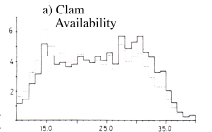
\includegraphics [width=1\textwidth] {clam1.png}
		\caption{}
        \end{subfigure}
        \space
        \space
        \begin{subfigure} [h] {0.3\textwidth}
                \centering
                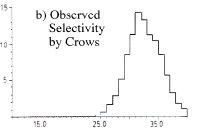
\includegraphics [width=1\textwidth] {clam2.png}
		\caption{}

        \end{subfigure}
	\space
	\space
	\begin{subfigure} [h] {0.3\textwidth}
                \centering
                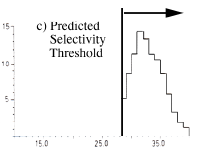
\includegraphics [width=1\textwidth] {clam3.png}
		\caption{}

        \end{subfigure}
\end{figure}

As we can see from (b) and (c) in fig \ref{fig:clams}, predicted behaviour seems to closely match observed behaviour. This kind of model, however, considers the disposition of prey in the environment to be random but, sometimes, prey items seem to have a patchy distribution (Sinevro 2006). In this case, an animal will have to travel between patches before it can start exploiting a new one. This creates two variables according to which an animal has to "make its decision" in order to maximise its rate of gain. The first one is the time spent within a patch to feed, and the second one is the time spent travelling between patches in which, crucially, the animal doesn't gain any energy and instead consumes it. A formula that effectively models this choice is:

\begin{equation*}
\emph{Rate of energy gain} = \frac{\emph{Energy}}{ \emph{Time}} = \frac {\emph{Energy or Load Size}}{ \emph{(Travel time to patch + Foraging time to patch}}
\end{equation*}

Also known as "\textbf{Charnov's Marginal Value Theorem}" which generates an energy gain function like the one on the left. Here, we can see how there are two main areas delimiting the Cartesian space, the first one (on the left side of the curve) is the potential time the animal has to spend in between patches, whereas the second one is the potential time spent feeding in a single patch. An optimal allocation of time in foraging for this rate of gain will be represented by the tangent to the curve as shown in the graphs on the right. The red line is the tangent and the point of intersection with the curve determines the in-patch time that would be optimal for an animal to spend feeding.

\begin{figure} [!ht] 
	\centering
           \makebox[\textwidth][c]{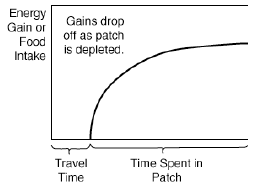
\includegraphics[width=0.4\textwidth]{gain1.png}}
	\caption{An energy gain function}
           \label{gain1}
\end{figure}

The aim of this proposal is evaluate subjects' innate ability to reproduce similar behaviours while foraging for information rather than for food. To do this, the context of a gold digging strategy game has been chosen, in order to remove all proximal cues that might depend on the user's previous experience. In this environment, the user will have to perform the same kind of cost vs. benefit choices, however, he would not be able to adopt the strategies he consciously would. Following I discuss a paper by Pirolli \& Card on Information Foraging which seems to support this intuition proposing experimental evidence and mathematical models.  "

\begin{figure}[!h]
        \centering
	\caption {The optimal rate of gain}
	\label{fig:gain tangent}
        \begin{subfigure} [h] {0.49\textwidth}
                \centering
                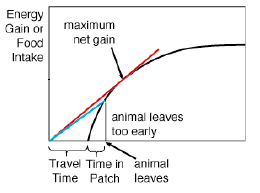
\includegraphics [width=1\textwidth] {gain2.png}
        \end{subfigure}
        \space
        \space
        \begin{subfigure} [h] {0.49\textwidth}
                \centering
                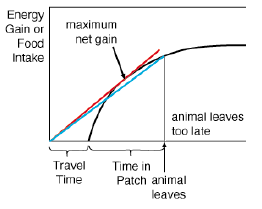
\includegraphics [width=1\textwidth] {gain3.png}
        \end{subfigure}
\end{figure}

\subsection{Information Foraging Theory}

Pirolli \& Card seem to start from the assumption that there are many similarities between the techniques adopted by animals foraging in the wild and the ones adopted by people in "Information Foraging". Because of the structure of today's society, in fact, it is not for food that we forage for. Food is usually readily available almost anywhere  human settlements can be found, however, to purchase it, we need to engage in a "complex tributary of cultural tasks that engage our physical and social environments" (Pirolli \& Card  1995) which demand us to develop numerous "information-based" strategies, in order to earn a living. Pirolli \& Card begin by explaining that our adaptive success seems to be increasingly dependent on our mastery of techniques of information-gathering, sense-making, decision-making and problem-solving strategies. In turn, they claim, this leads us to implement strategies which are similar to the ones seen in foraging behaviours of animals in the wild. Here, we can observe patterns in food foraging behaviours which aim at maximising the energy intake while minimising the amount of energy spent while foraging. 

In other words, our lives are increasingly dependent on the ways in which we organise and retrieve information in order to use it effectively to navigate and survive today's social (and sometimes physical) landscape. Pirolli \& Card go on to claim that, the Information Foraging theory's main tenant is that:  "when feasible, natural information systems evolve towards stable states that maximise gains of valuable information per unit cost. Cognitive systems engaged in information foraging will exhibit such adaptive tendencies" (Pirolli \& Card  1995). 

As a consequence, it is to be expected that people will modify their information foraging strategies as well as the structure of the environment itself, whenever possible, to "maximise the rate of gaining valuable information" (Pirolli \& Card  1995). Better strategies will be the ones that will allow someone who adopts them to yield more information per unit cost. Furthermore, it is also expected that these strategies will evolve through time, in order to reach a seemingly stable state that maximises the potential gains. 

The process of analysing the development of this kind of behaviour, is called "adaptation analysis". This kind of analysis is conducted here, as well as in biology, through the use of "optimisation models" to study the design features of organisms and artefacts. Optimisation models include three major components:

\begin{itemize}
	\item \textit{Decision assumption}, determine how much time is to be spend analysing a certain collection of information as well as which kind of content is worthwhile pursuing.
  	\item \textit{Currency assumptions}, determine how the choices made through decision assumptions are to be evaluated. In the context of Information Foraging, the relevant currency will be amount of relevant documents found, as opposed to the amount of energy gained in food foraging strategies.
  	\item \textit{Constraint assumptions}, determine what kind of limits will apply to the relationship between decision and currency assumptions. In Information Foraging, these include (but are not limited to) previous knowledge, available technology and task structure.
\end{itemize} 

These models allow us to construct a framework for the evaluation in Information Foraging, however, it is not to be expected that any single individual will fully be conscious and even evolve towards, an optimal awareness and implementation of these models. These models simply outline the possibility of "an advantageous adaptation if not blocked by other forces”. 

The main decision an organism has to make in its foraging endeavours (being it for food or for information) is determined by a problem of "Enrichment vs. Exploitation” of a certain "patch” of relevant documents (or food). The careful weighing of one against the other, will, in turn, determine its searching behaviour, comprehensive of "in-patch” and "between-patch behaviours”.  When we decide to "enrich” a certain patch of information, we engage in certain "enrichment strategies” which are meant to maximise the amount of relevant information per unit of cost that we are able to get from a patch. However, the adoption of these strategies themselves has a cost which should be considered when making the decision to move to a different patch and select a new set of documents. There are two main "in-patch” enrichment strategies. 

The first one is based on producing information packages that yield better results. This involves strategies like developing or acquiring better search tools, as well as spending time mastering them. The second one is based on filtering the incoming information into relevant topics or according to other decisional criteria devised by the foragers and that they came to realise as useful to their foraging needs. 

Another way foragers can increase their gain in yielded by their foraging behaviours is by using "between-patch” enrichment strategies. These are also of two kinds. The first one is constituted by what Pirolli \& Card call "scent-detection strategies”. These strategies are based on the identification of proximal cues in the environment in order to make a choice on whether it would be fruitful to explore a certain "patch” or move to another one based on detection of proximal cues. In the context studied by Pirolli \& Card, this translates into identifying the relevance of a certain document, or group of documents by, for instance, its title and payoff, perceived clarity of writing or length. 

A second kind of in-patch enrichment strategy is based on reducing the cost of getting from one information patch to another. While this is usually impossible for animals in the wild, because it involves modifying the environment, it is instead a very efficient way for information foragers to improve the rate of gain per unit cost. In the example proposed by Pirolli \& Card this is shown in the re-organisation of the workspace of an employee whose job is to write a Business Intelligence Newsletter. The subject of their experiment, in fact, organised the different areas of his office, in order to minimise the time spent searching for relevant document by disposing the material he knew he would need more frequently, the nearest to his working station.

For the purpose of this proposal it is also important to consider the conventional models of foraging on which Information Foraging Theory is based. As it can be expected, to provide an efficient model of foraging, we will have to take into account equations which model both in-patch and within-patch behaviours. Given what previously stated, Pirolli \& Card start by characterising the rate of gain of valuable information per unit cost R as the ratio of the total net amount of valuable information gained $G$ divided by the total amount of time spent between patches $T_B$ and exploiting within patches $T_W$ a

\begin{equation}
R = \frac{G}{T_B + T_W}
\label {eq:main}
\end{equation}

Notably, this equation assumes that (1) "the total amount of information gained can be represented as a linear function of between-patch foraging time:

\begin{equation}
G = \lambda T_B g
\end{equation}

And that (2) “the total amount of within-patch time can be represented as:

\begin{equation}
T_W = \lambda T_B t_W
\end{equation}

This, in turn, gives Holling's Disc Equation:
\begin{equation}
\begin{split}
 R = \frac{\lambda T_B g}{T_B + \lambda T_B t_W} \\
= \frac{\lambda g}{1 + \lambda t_w}
\end{split}
\end{equation}

This formulation, however, "addresses the problem of allocation of time between in-patch vs. between patch under certain strong assumptions". Because of this, Pirolli \& Card have to devise their own interpretation which takes in to account that "(a) there might be different kinds of patches and (b) the total gains from a patch depend on the within-patch foraging time which is under the control of the forager. For this reason they have to include a value \emph{i} representing the type of patches encountered at a rate of $\lambda$ i and a value $t_wi$ representing the \emph {policy} adopted by a forager on how much time to spend within each patch. The total gain can then be represented as the sum of all the values of \emph{i} between 1 and P.

\begin{equation}
\begin{split}
G = \sum_{\substack{i=1}} \lambda_i T_B g_i (t_{wi}) \\
= T_B  \sum_{\substack{i=1}} \lambda_i g_i (t_{wi})
\end{split}
\end{equation}

In the same way, the total amount of time spent within patches could be represented as:

\begin{equation}
\begin{split}
T_W = \sum_{\substack{i=1}} \lambda_i T_B t_{wi} \\
= T_B  \sum_{\substack{i=1}} \lambda_i (t_{wi})
\end{split}
\end{equation}

Combining these two equations according to (eq. \ref{eq:main}) gives us:

\begin{equation}
\begin{split}
R = \frac{T_B \sum_{\substack{i=1}} \lambda_i g_i (t_{wi})}{T_B + T_B  \sum_{\substack{i=1}} \lambda_i t_{wi} } \\
= \frac{\sum_{\substack{i=1}} \lambda_i g_i (t_{wi})}{1 + \sum_{\substack{i=1}} \lambda_i t_{wi} }
\end{split}
\end{equation}

This last equation is what Pirolli \& Card call the \emph"patch model for information foraging" which takes into account patches that yield different kinds of gain functions as well as different strategies to exploit them.

\begin{figure} [!ht] 
	\centering
           \makebox[\textwidth][c]{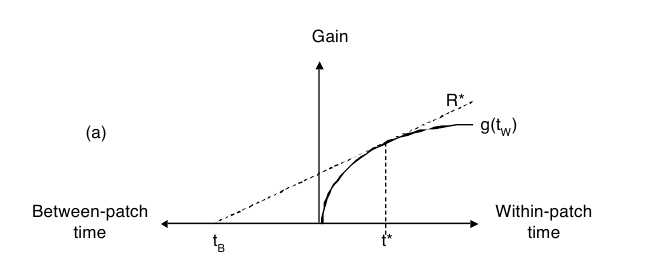
\includegraphics[width=0.8\textwidth]{enrichment1.png}}
	\caption{(a) - The Graph illustrates Charnov's Marginal Value Theorem  where t* denotes the optimal amount of time spent within-patch given the intersection between the gain function $g(t_w)$and the tangent passing from $t_B$ (the time spent between patches)}
           \label{gain1}
\end{figure}
\begin{figure} [!ht] 
	\centering
           \makebox[\textwidth][c]{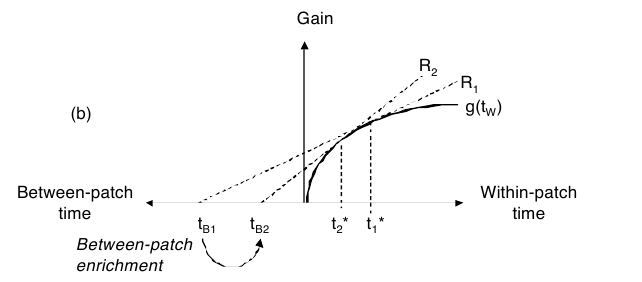
\includegraphics[width=0.8\textwidth]{enrichment2.png}}
	\caption{(b) - Shows the changes generated by the adoption of between-patch enrichment strategies. The tangent to the gain function $g(t_w)$ passing from $t_{B2}$  determines that the optimal amount of time to spend in a given patch is now $t_2*$ . The forager is now able to afford to spend less time in each patch.}
           \label{gain1}
\end{figure}
\begin{figure} [!ht] 
	\centering
           \makebox[\textwidth][c]{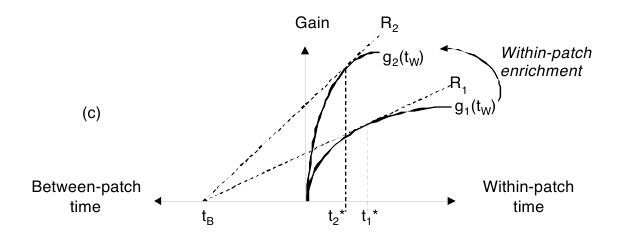
\includegraphics[width=0.8\textwidth]{enricment3.png}}
	\caption{(c) - Shows the changes generated by the adoption of within-patch enrichment strategies. The new gain function $g_2(t_w$) has a higher rate gain which  allows foragers that spend the same amount of time between patches $t_B$ will be able to reap more results in a shorter time.}
           \label{gain1}
\end{figure}

Figures (a), (b) and (c) are the graphical representation of the functions presented in the previous section according to Charnov's Marginal Value Theorem, they model the problem of allocation of time between in-patch vs. between-patch strategies. Here, between-patch search times $t_B$ , $t_{B1}$ and $t_{B2}$ generate different tangents to the $g(t_w)$ gain function which, in turn, determines the optimal rate of gain $R$. The outside of the curve on the x axis represents between-patch time while, the inside of it, represent within-patch time. To determine the optimal rate of gain $R*$ one draws the tangent line to the gain function $g(t_w)$ and passing through $t_B$ . The point of tangency will determine the "optimal allocation of within-patch foraging time $t*$".  

This means that, the more time is spent between-patch, the less a forager will find it beneficial to spend time exploiting a given patch, always depending on the gain function g(tw). In Figure 2, in fact, we see the effects of a between-patch enrichment like the one described previously (office re-disposition) which sets the optimal rate of gain in such a way that it will be more beneficial for the forager to spend more time within-patch to exploit it. Finally, in Figure 3 we can see the effect of within-patch enrichment (for instance, making information packages that yield better results). As we can see, within-patch enrichment, changes the gain function g(tw) determining higher gains per unit of time spent within-patch.

The objective of the experiment outlined in this proposal, is to be able to evaluate the strategies adopted by subjects in order to reach an optimal rate of gain and to analyse how they are able to choose between within/between-patch enrichment strategies to better their rate of gain per unit cost. 


\section{Previous studies}
\subsection{Searching behaviour}
\subsection{Gamification}

%%%%%%%%%%%%%%%%%%%%%%%%%%%%%%%%%%%%%%%%%%%%%%%%%%%%%%%%%%%%%%%%%%%
\chapter{Design}\label{design}

The design of Gold Digger went through different iterations through the course of its development (see 4.2 Heuristic Evaluation), however some design choices were made in order to keep the user experience consistent throughout the website and enhance clarity and ease of use.

\textbf{Separation between "game pages" and "site pages"}

Because Gold Digger is both a website and a game, it seemed appropriate to somehow separate the "game environment" from the more "site-like" features and pages, while still maintaining a certain degree of coherence between them. "Game pages" are the ones immediately relevant to the game in itself, the ones that the user will most likely enter while playing Gold Digger. These are: \textbf{the Game/Mine page, the General Shop page, the Home Page} and \textbf{the World Map Page}. The other pages are said to be "site pages" and they include pages like the About page and the Leaderboards, which a user is not very likely to access while in the middle of a play through. Furthermore "game pages" all require the user to be logged in to be accessed while the "site pages" do not. 
\\*
Notwithstanding this distinction, the user experience is not disjointed thanks to prominent recurring elements such as the nav bar on the top of the page and the landscape headline showing the name of each page.

\section{Site Map}

Navigation through the website is aided by a navbar located at the top of every page (with the exception of the 'game over' and 'end of the day'
pages). 
\begin{figure} [h] 
	\centering
           \makebox[\textwidth][c]{
\includegraphics[width=1\textwidth]{nav.png}}
	\caption{Gold Digger nav bar}
           \label{navbar}
\end{figure}

From the navbar the user will be able to reach the following pages:

\begin{itemize}
  	\item The main page (by clicking on 'Gold Digger')
  	\item The World Map page (if signed in)
	\item The Leadeboards
	\item The About page
	\item The 'How to Play' / Tutorial page
	\item The 'Achievements' page
  	\item The User Profile page (if signed in)
\end{itemize} 

finally, the user will also be able to logout at any moment by using the 'Logout' button on the top right. However, if the user is currently in one of the mines,
clicking on one of these links will result on a warning message being displayed that will alert users that the gold gathered during the day will be lost if they leave
the mine before exhausting the time at their disposal and reaching the end of the day. 

\subsection{Home, Registreation and Login}


\begin{figure} [h] 
	\centering
           \makebox[\textwidth][c]{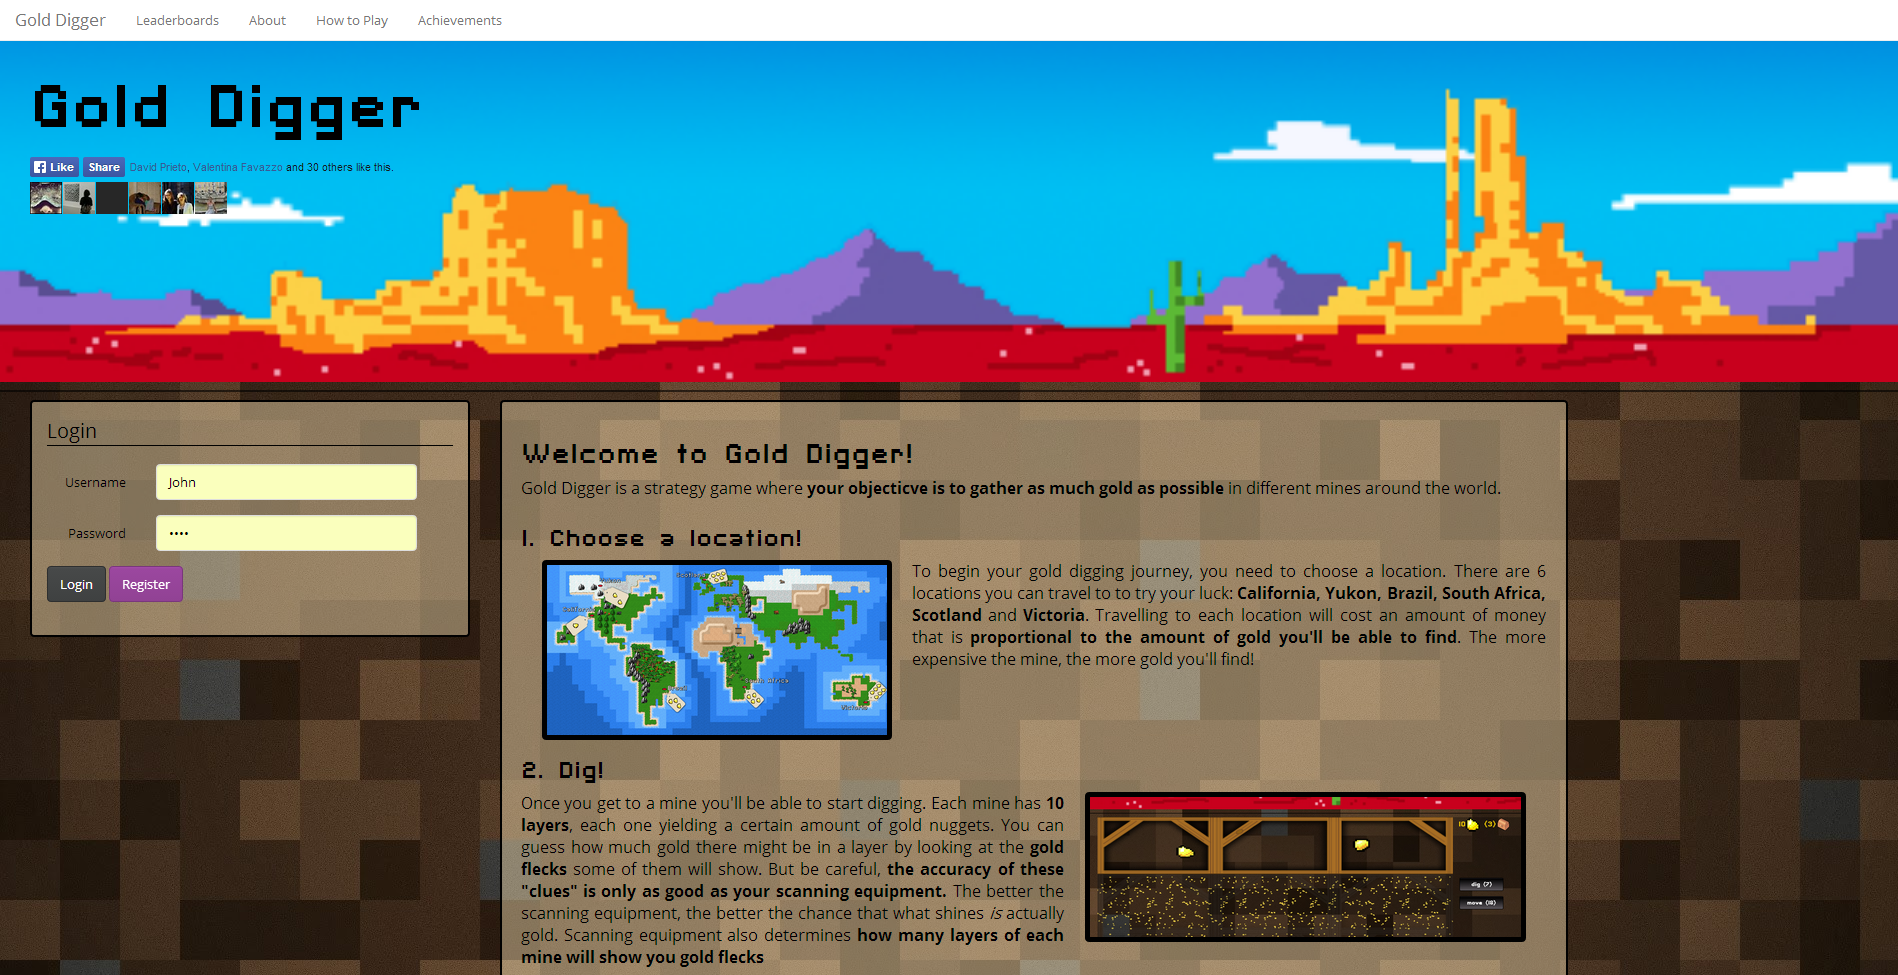
\includegraphics[width=1.2\textwidth]{homescreen.png}}
	\caption{Home Page}
           \label{homepage}
\end{figure}

On the landing page (homepage) users will be presented with a short \textbf {five-point explanation} of the game to quickly explain the mechancs of the game so that
users could start playing as soon as poosible. To so this, they will have to login through the form on the left or register by clicking on the 'Register' button. 
\begin{figwindow}%
[0, r, 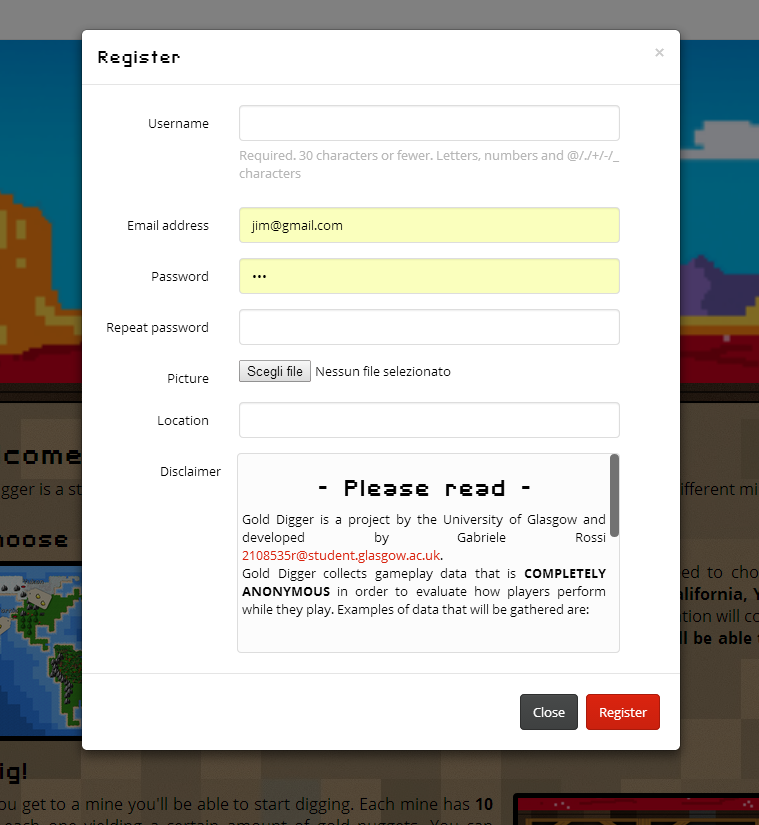
\includegraphics[width=.5\textwidth]{register.png},%
{ Registration modal}]
Clicking on the \textbf{ 'Register'} button will trigger a modal asking users to create a new username and password, as well as optionally entering their location and user
picture. Finally, the modal displays a disclaimer in order to both make sure that the users are aware of the limitations of accessing the website and its purpose. 
Users who wish to have more information about Gold Digger are redirected to the 'About' page or offered a link to directly write an email to the developer.
\\
Finally if a user enters wrong details or forgets to fill in a required field, (both for registration and login) an appropriate error message is clearly displayed for the user to see and try again. 
At present there is no limit to the number of attempts a user can make at logging in or registering.

\end{figwindow}

\subsection{World Map}

\begin{figure} [h] 
	\centering
           \makebox[\textwidth][c]{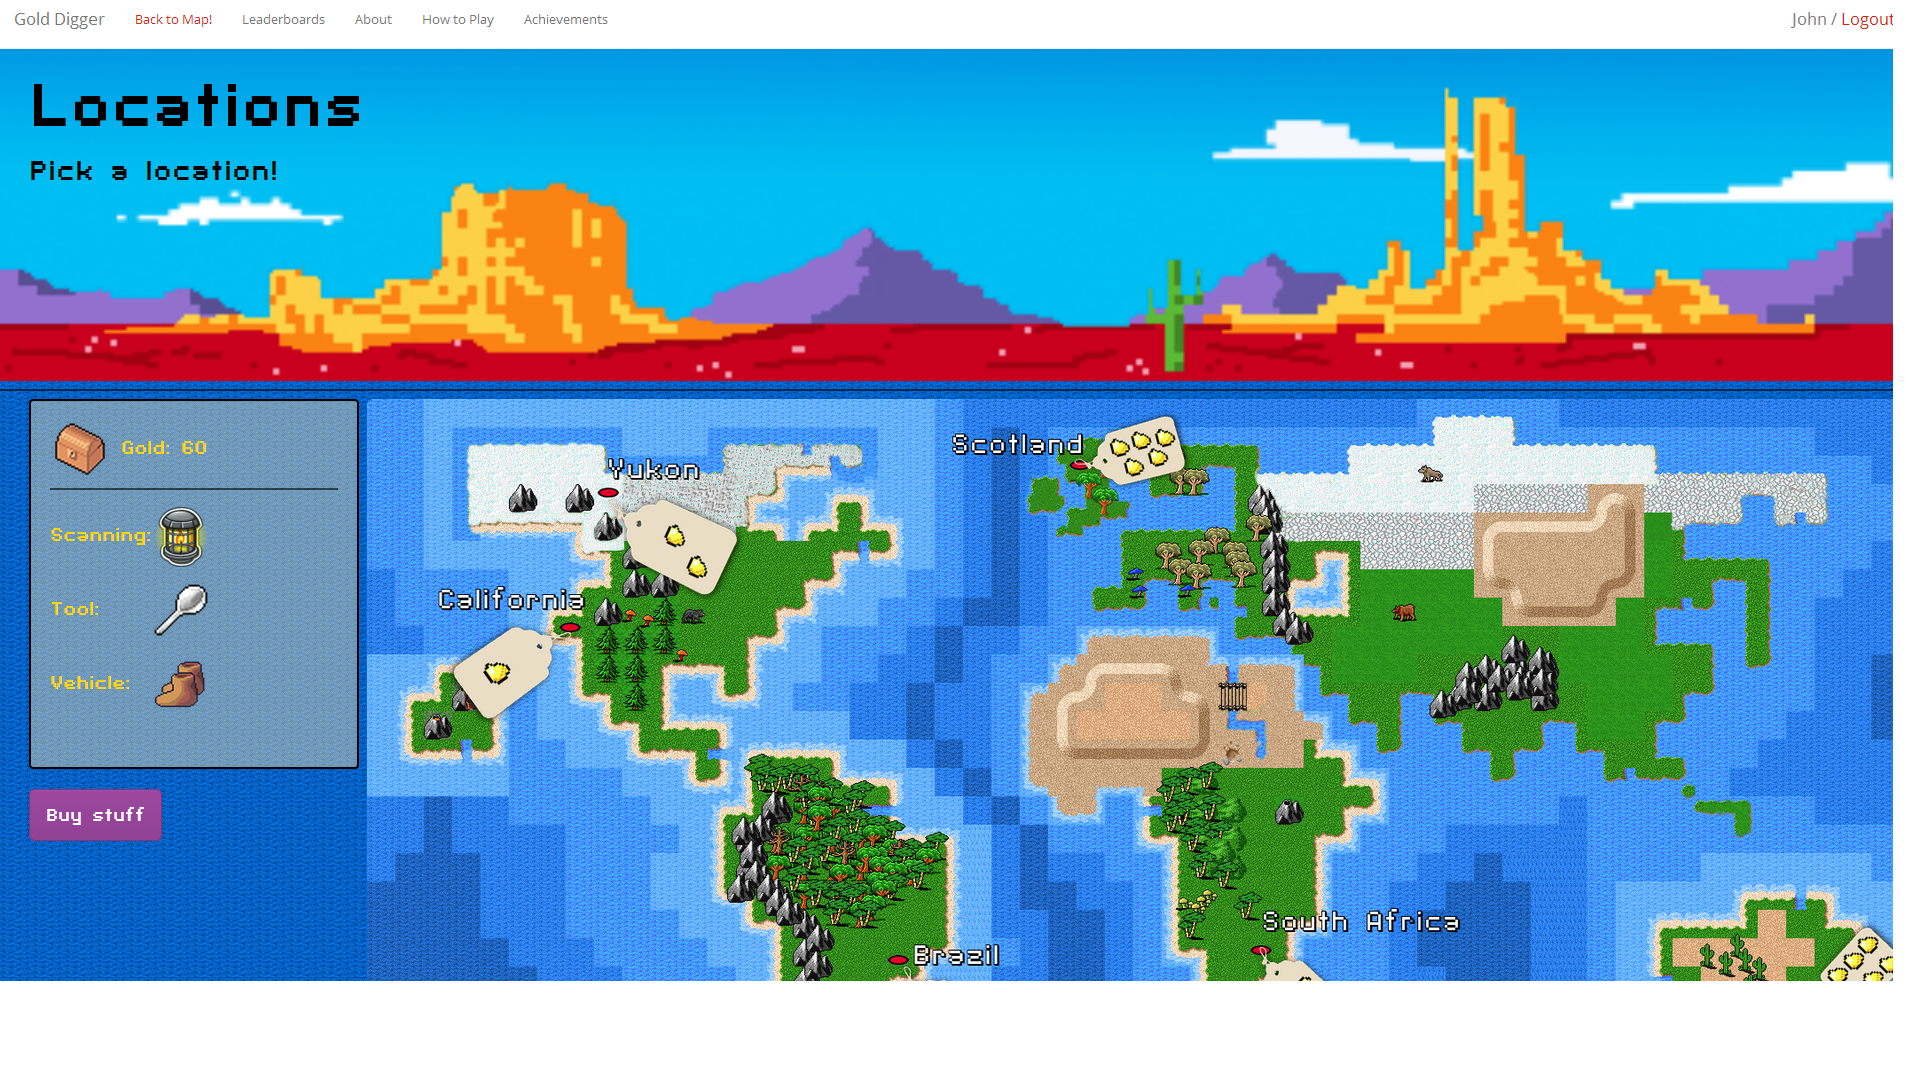
\includegraphics[width=1.2\textwidth]{worldmap.png}}
	\caption{World Map}
           \label{worldmap}
\end{figure}

Once users have registerd or have been logged in, they are automatically redirected to the world map so that they can start playing immediately. 
On the left of the page, users can see the euqipment and the amount of gold they have at the moment. The side item panel appears on the left column of the page, once the user has logged in. The panel shows the items that users have equipped, together with the total amount of gold in their possession. By hovering over each one of the items a tooltip will appear, showing the essential stats of each item. The presence of the side item panel has the function of both confirming the users that they are logged in and  reminding them that their game session has started  contributing to the uniformity of the user experience.
\begin{figwindow}%
[0, l, 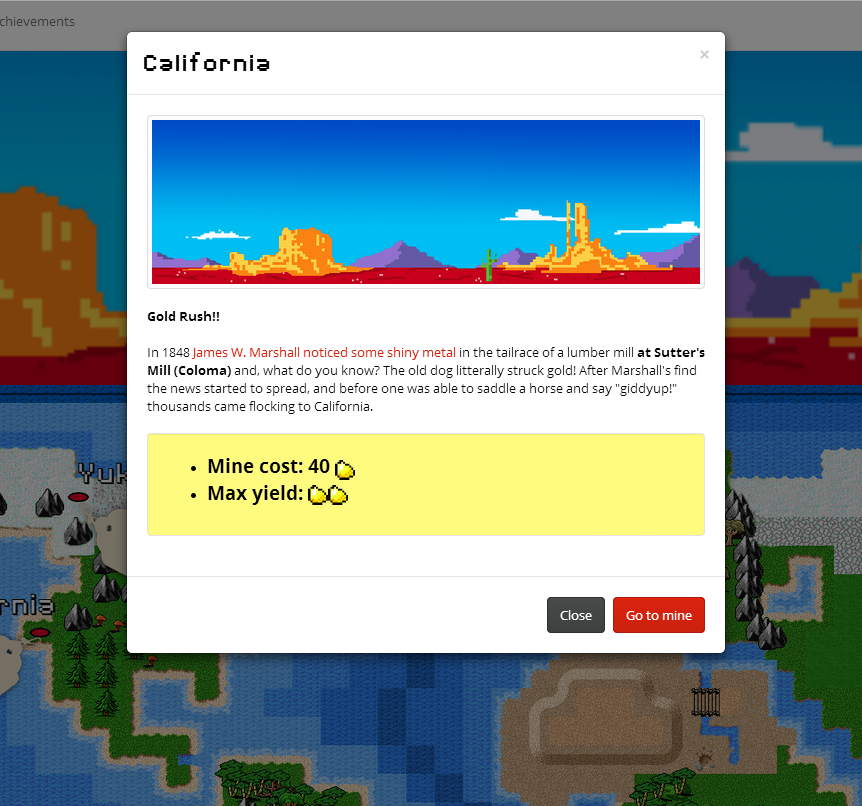
\includegraphics[width=.4\textwidth]{cali.png},%
{ California modal}]
 On the right hand side of the page users can access any of six locations: \textbf{California, Yukon, Brazil, South Africa, Scotland} and \textbf{Victoria}. 
Clicking on any of the locations will trigger a modal that displaying the scenery of the particular mine, some information about the gold digging history in that region (with links to Wikipedia articles), the cost of the mine and the amount of gold the user can expect to find. Starting from California and ending with Victoria, each mine is more expensive than the previous one 
but it also have a potentially higher gold yield. It is up to the player to enter the right mine at the right time.
\end{figwindow}

\subsection{Game Screen}
\begin{figure}[h] 
	\centering
           \makebox[\textwidth][c]{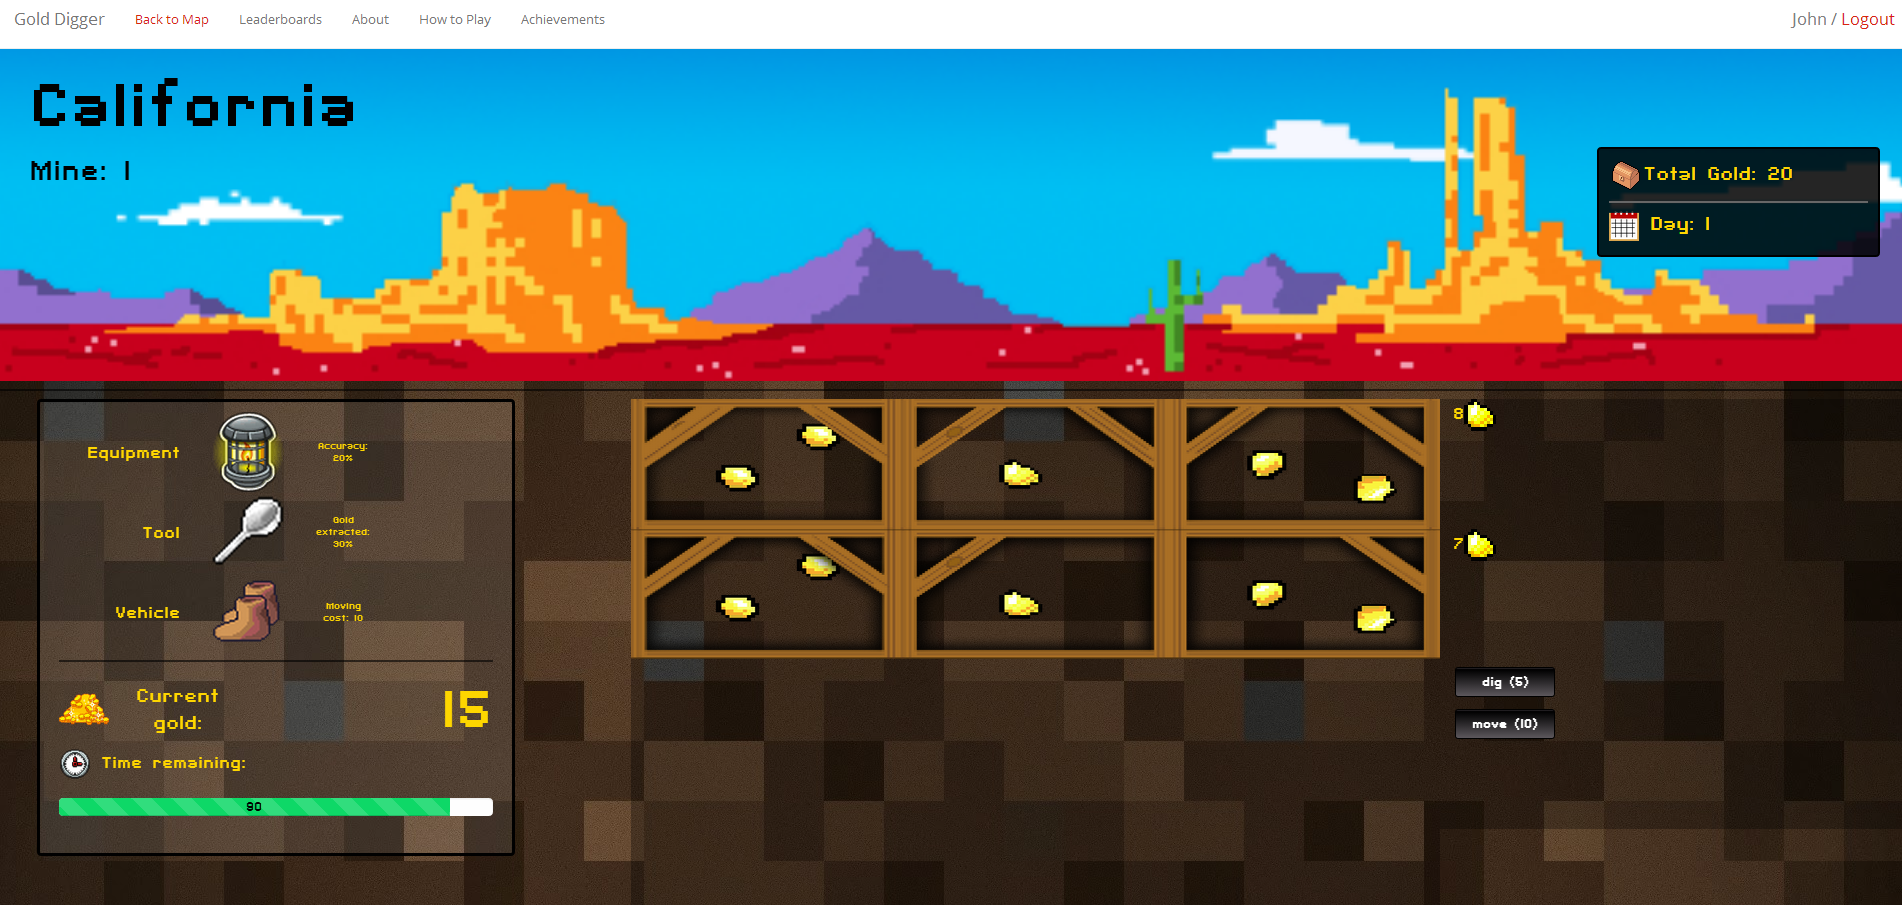
\includegraphics[width=1.2\textwidth]{mine.png}}
	\caption{Mine}
           \label{mine}
\end{figure}

Once the users enter a mine, the appropriate amount of gold is removed from the total and they can start digging. Each mine presents a similar structure, except for the landscape and the
amount of gold that can be found in each layer. On the top of the page we can see the landscape picture and the name of the location, as well as the number of mines that the user has dug into during the present day. As previously noted, on the left, we can find the equipment panel, in the middle we have the mine shaft and on the right have the \textbf {'Dig'} and \textbf{'Move'} as well as the yield of each layer that has been already dug. The left side panel contains here some more information than it does in the other pages where it appears:
\begin{itemize}
  	\item \textbf{Current gold}: the amount of gold gathered during the present day.
  	\item \textbf{Time remaining}: the amount of time (in units of time) remaining before the end of the day.
\end{itemize} 
Furthermore, because the left side panel's position is fixed, it will follow users as they get deeper and deeper in the mine, allowing them to always keep an eye on the game state without having to go back to the top of the page to check how many units of time they have left before the end of the day. Because the 'Current gold' is summed to the 'Total Gold' only at the end of the day, the total amount of gold, together with the number of days users have been digging without encountering a game over, is displayed in a small box on the top right of the page.
 The options available to the user and an example of gameplay are detailed in section 3.2.

\subsection{General Store}

\begin{figure} [h] 
	\centering
           \makebox[\textwidth][c]{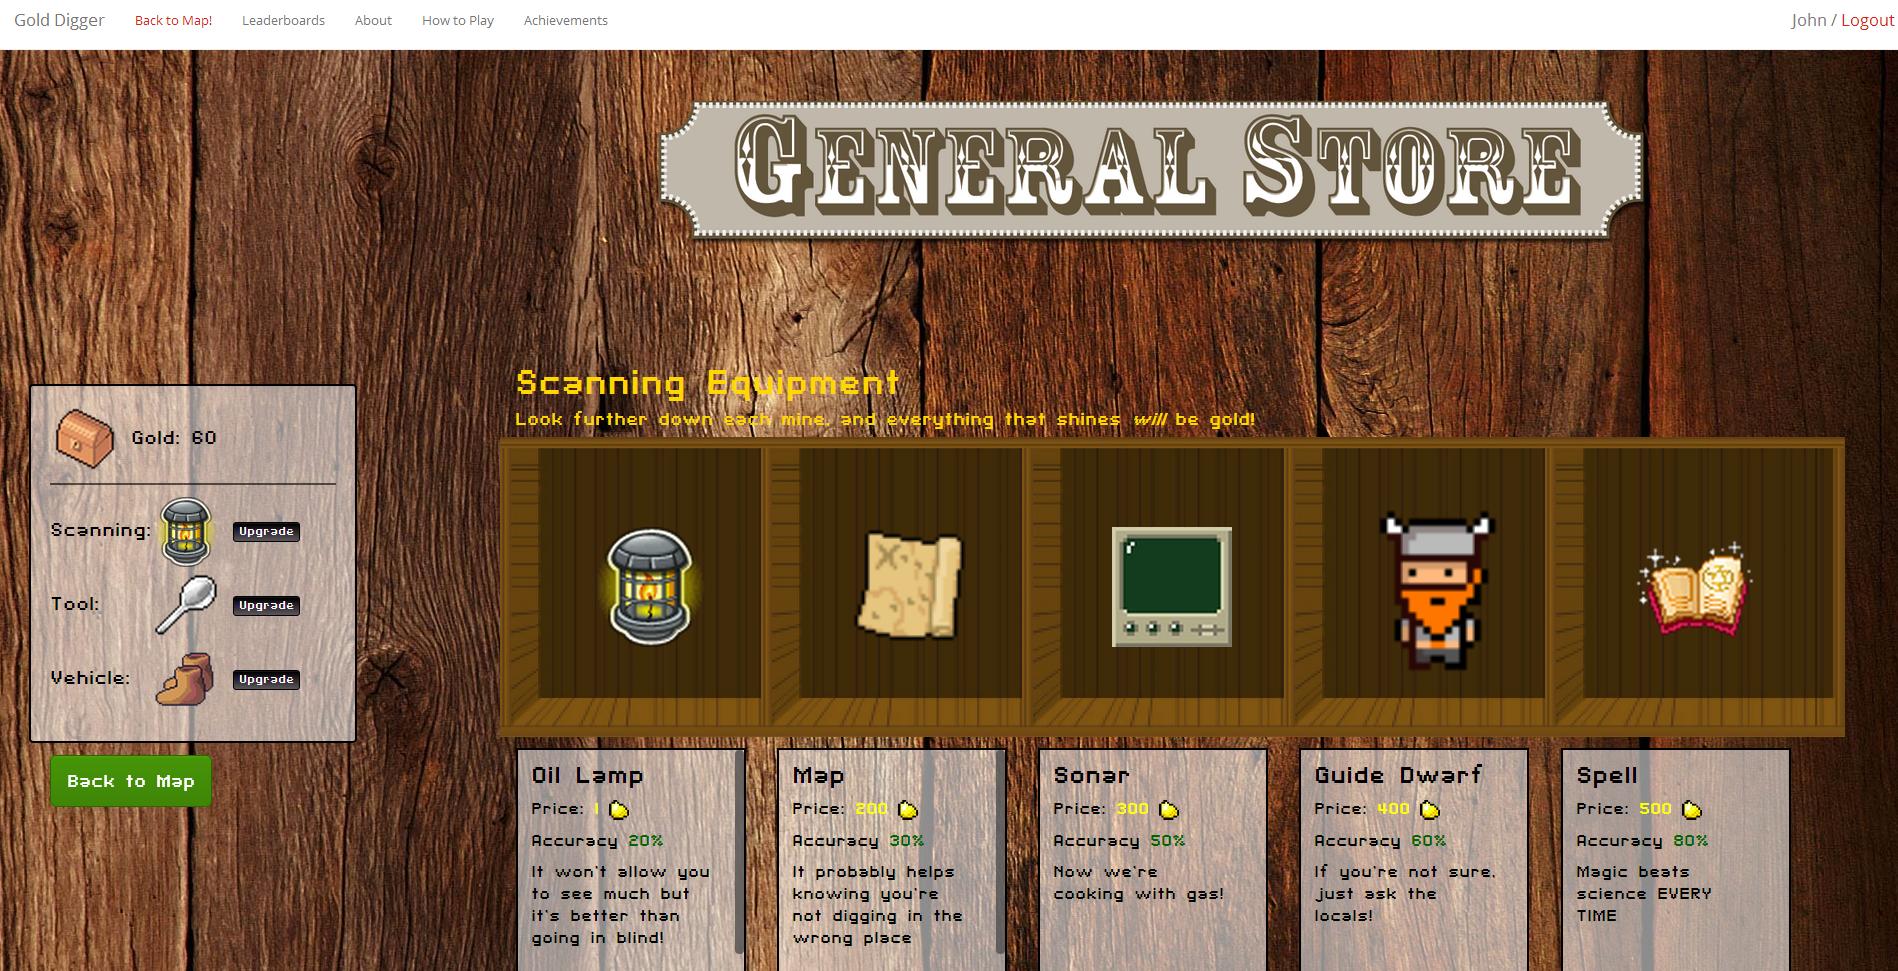
\includegraphics[width=1.2\textwidth]{generalstore.png}}
	\caption{General Store}
           \label{fig: generalstore}
\end{figure}

At the end of each day (by clicking on \textbf{'shop'}), or from the world map screen (by clicking on \textbf{'Buy stuff'}), users can access the \textbf{General Store} (see fig. \ref{fig: generalstore}). From here they are able to browse and purchase new items to help them in their digging. There are three groups of objects that the user can choose from \textbf{Scanning Equipment, Digging Equipment} and \textbf{Vehicles}. Each of these groups contains five different items with different cost and stats. Users are able to see the image associated with each item as well as its cost,  stats and a short description in the small tex box underneath. If users decide to upgrade one of their item groups (Scanning, Digging or Vehicle) they can do so by clicking on the \textbf{'Upgrade'} button. At this point they will be presented with a small modal that reviews the item's stats, together with its picture, asking the user to confirm the purchase. If the users don't have enough gold to make the purchase, or if the purchase would cause them to not have enough money to enter the cheapest mine, an appropriate alert message is displayed, explaining why the purchase is not possible.

The choice to allow users to \emph{upgrade} rather that \emph{buy} items has been made because each of the items is better than the previous one in every respect and thus there is no reason why a user would chose to equip an item that they previously purchased, since this would not bring any advantage at all. For instance, with digging tools, their cost, dig cost (the amount the user has to pay in time units to dig once) and extraction power (the percentage of gold that the user will be able to extract given a certain yield), are all increased from the least, to the most expensive. However, it would be easy to add items that have different combinations of these parameters and add, for example, a digging tool that, at a higher cost per dig also returns a higher percentage of gold.
Finally, upon purchase, the new item is immediately added to the left side panel and the appropriate amount of money removed from the user's total through an AJAX call.

 \subsection{Leaderboards}

\begin{figure} [h] 
	\centering
           \makebox[\textwidth][c]{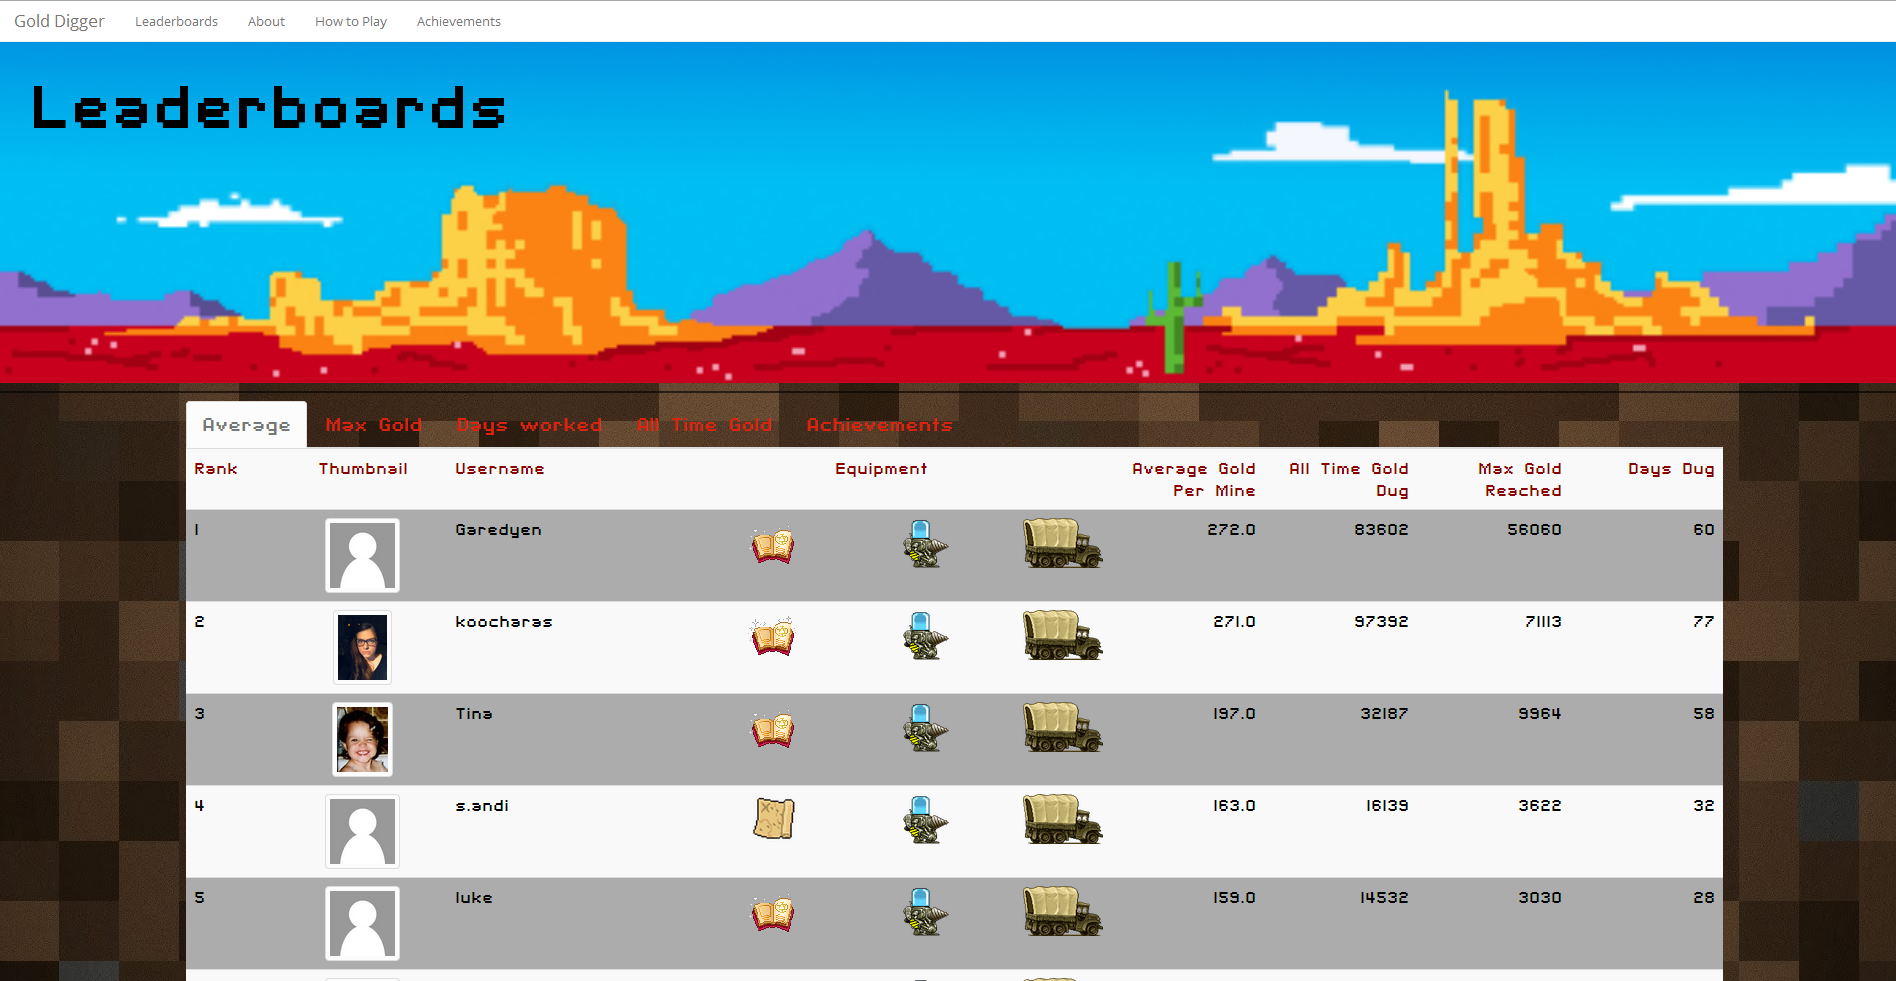
\includegraphics[width=1.2\textwidth]{leaderboards.png}}
	\caption{Leaderboards}
           \label{fig: leaderboards}
\end{figure}

On the \textbf{Leaderboards} (see fig. \ref{fig: leaderboards}) page, users are able to check their performance and compare it to the other players'. There are four parameters by which users can be ranked, plus an achievements board that has no specific ranking criteria: 

\begin{itemize}
  	\item \textbf{Average}: the total amount of gold ever dug by the player divided by the total amount of mines that were dug into.
  	\item \textbf{Max Gold}: the maximum amount of Gold ever dug (the maximum amount of gold ever reached)
	\item \textbf{Days Worked}: the total amount of days of digging completed by the player (not zeroed on game over)
	\item \textbf{All Time Gold}: the cumulative total amount of gold dug by the player  (not zeroed on game over)
	\item \textbf{Achievements}: shows the achievements gained by each player in no particular order (achievements are not ranked)
\end{itemize} 

Each row of the the tables (excluding the 'Achievement' table) diplays the following parameters: Rank, Thumbnail, Username, Equipment (showing the image for each of the three item groups), Average Gold per Mine, All Time Gold Dug, Max Gold Reached, Days Dug.

\subsection{Tutorial}

\begin{figure} [h] 
	\centering
           \makebox[\textwidth][c]{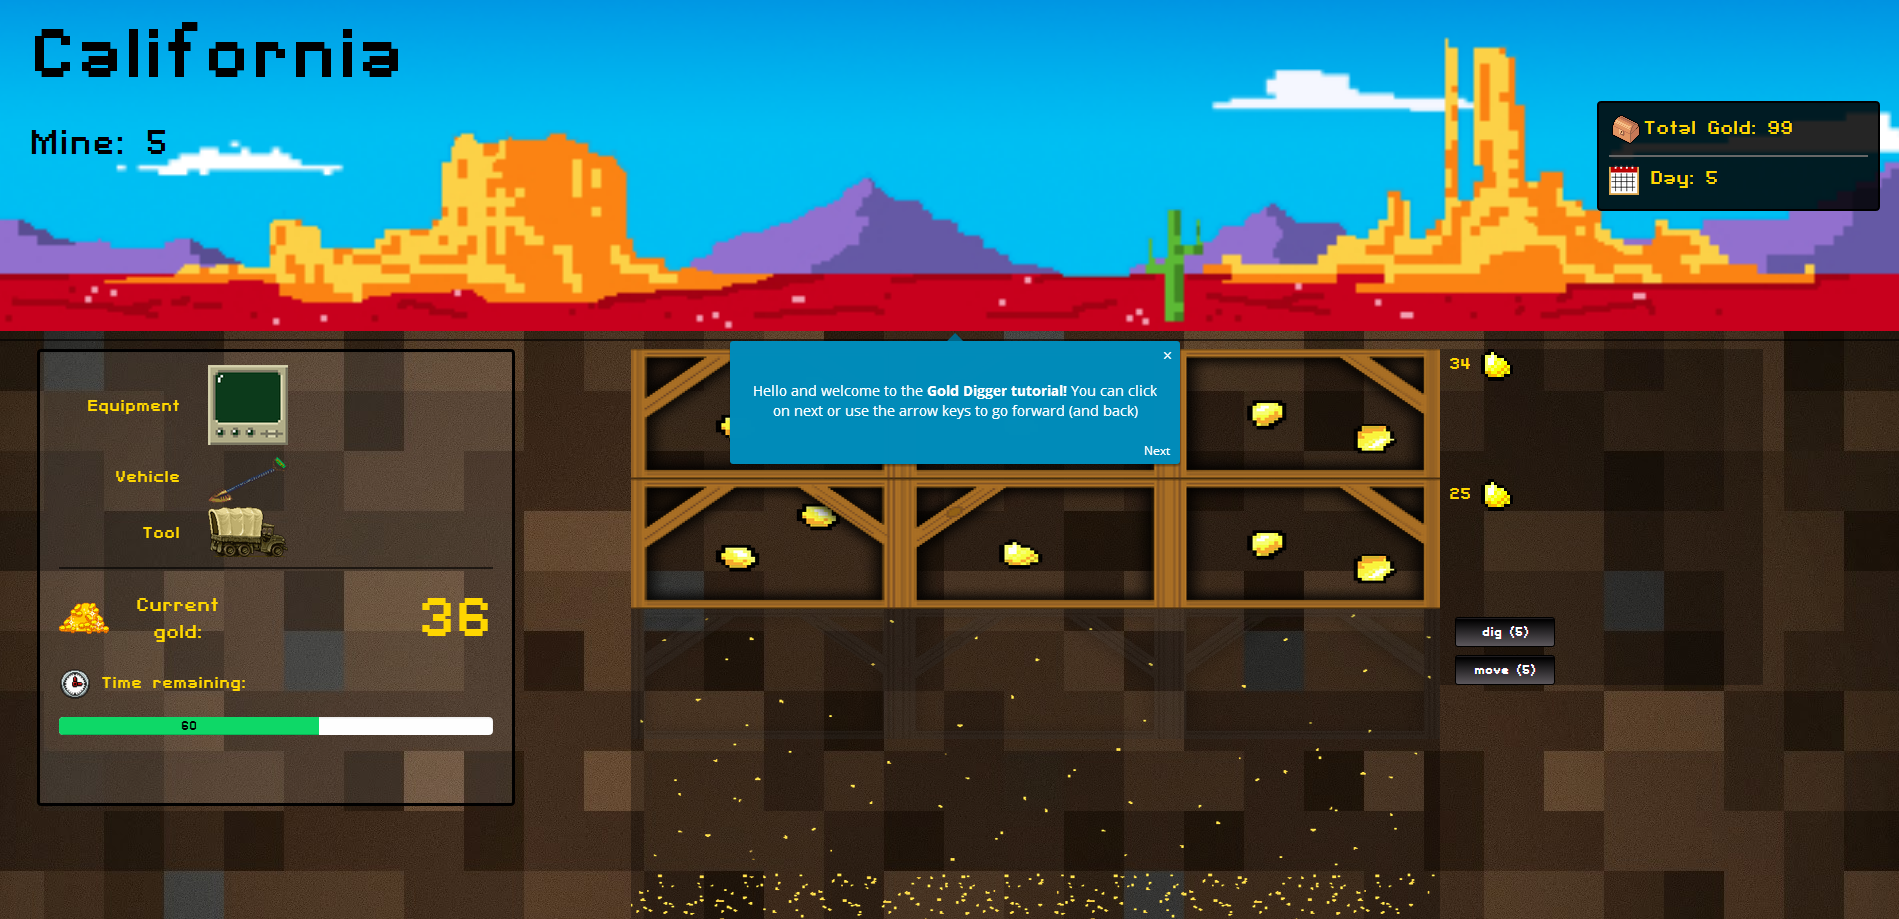
\includegraphics[width=1.2\textwidth]{tutorial.png}}
	\caption{Tutorial}
           \label{fig: tutorial}
\end{figure}

Because it is important for users to have a clear idea of the way the game works, all effort has been made to employ a visual approach that would be quick and easy to understand. To this end, upon entering, the \textbf{'How to Play'} page, a tour of the main game features is automatically launched. The javascript library \textbf{Trip.js} (see 4.4.6) highlights and points at the different parts of the game screen in order to get a quick visual explanation of the main game mechanics. Each of the labels has 'Next', and 'Previous' link, in order to let users go back to a previous point or skip explanations they already viewed.

\subsection{Achievements}

\begin{figure} [!hb] 
	\centering
           \makebox[\textwidth][c]{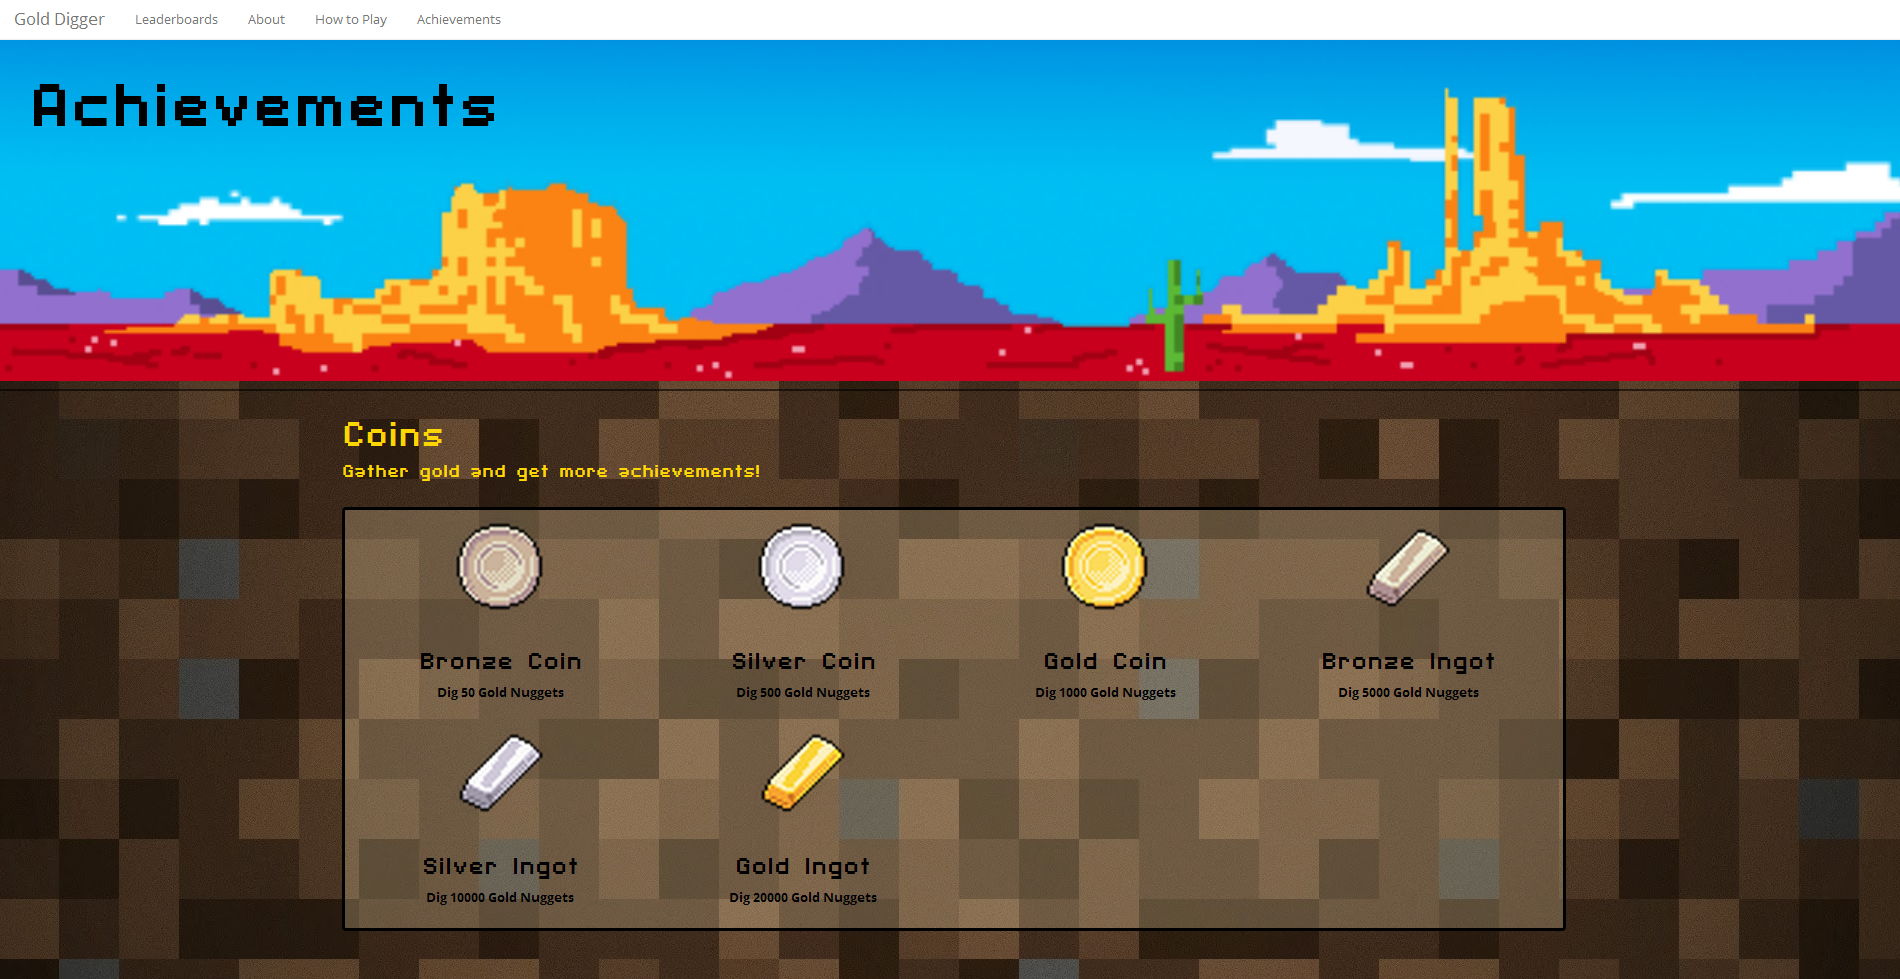
\includegraphics[width=1.2\textwidth]{achievements.png}}
	\caption{Achievements display}
           \label{fig: achievements}
\end{figure}

The \textbf{'Achievements'} page dispays all the achievemts badges together with their name, the condition that triggers them and their image. This page is needed in order for the users to be able to check which achievements they can aim for while playing. Two additional achievements (fig. \ref{fig: specialachievements}) are not displayed here and are given only under special conditions:

\begin{figure}[!h]
        \centering
        \begin{subfigure} [!h] {0.4\textwidth}
                \centering
                
\includegraphics [width=0.4\textwidth] {awesome.png}
                \caption{You helped testing!}
                \label{}
        \end{subfigure}
        \space
        \space
        \begin{subfigure} [!h] {0.4\textwidth}
                \centering
                
\includegraphics [width=0.4\textwidth] {banana.png}
                \caption{You found the Easter Egg!}
                \label{}
        \end{subfigure}
        \caption{Special Achievements}
        \label{fig: specialachievements}
\end{figure}

\begin{itemize}
  	\item \textbf{Awesomeness}: given to the people who tested the "beta" version of the site.
  	\item \textbf{Banana}: given to people who managed to find the game's Easter Egg
\end{itemize} 

Achievements ans special achievements have been incorporated in order to both add an extra game feature to Gold Digger which wouldn't change the game mechanics too much an to give players an incentive to keep playing, especially since there is no particular "winning condition", fulfilled which a player has completed the game.  

\subsection{About Page}

In this page, users are able to find  the developer and supervisor's contact details as well as reading about the reasons behind the creation of Gold Digger and acknowledgements of the authors of some of the material used in the site.


\section{Walkthrough}

\begin{figure}[!h]
        \centering
        \begin{subfigure} [h] {0.6\textwidth}
                \centering
                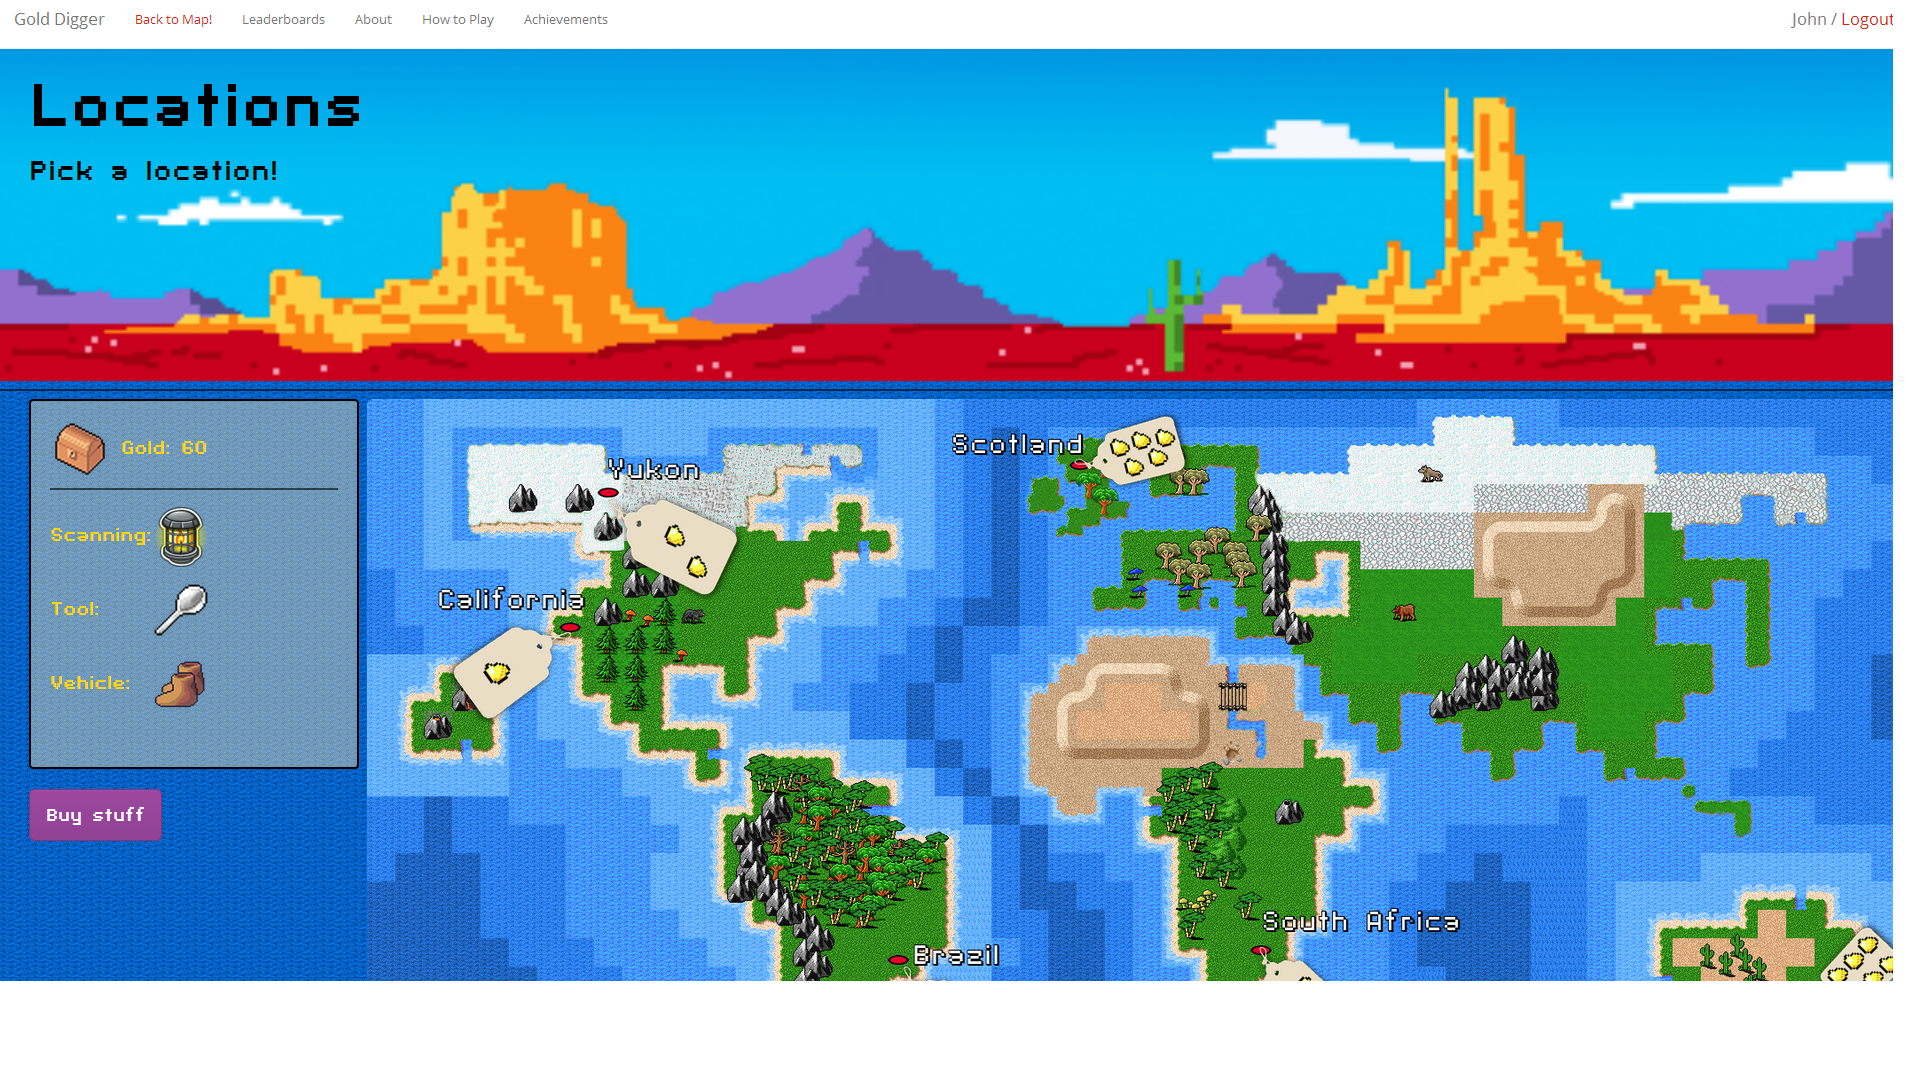
\includegraphics [width=1\textwidth] {worldmap.png}
        \end{subfigure}
        \space
        \space
        \begin{subfigure} [h] {0.3\textwidth}
                \centering
                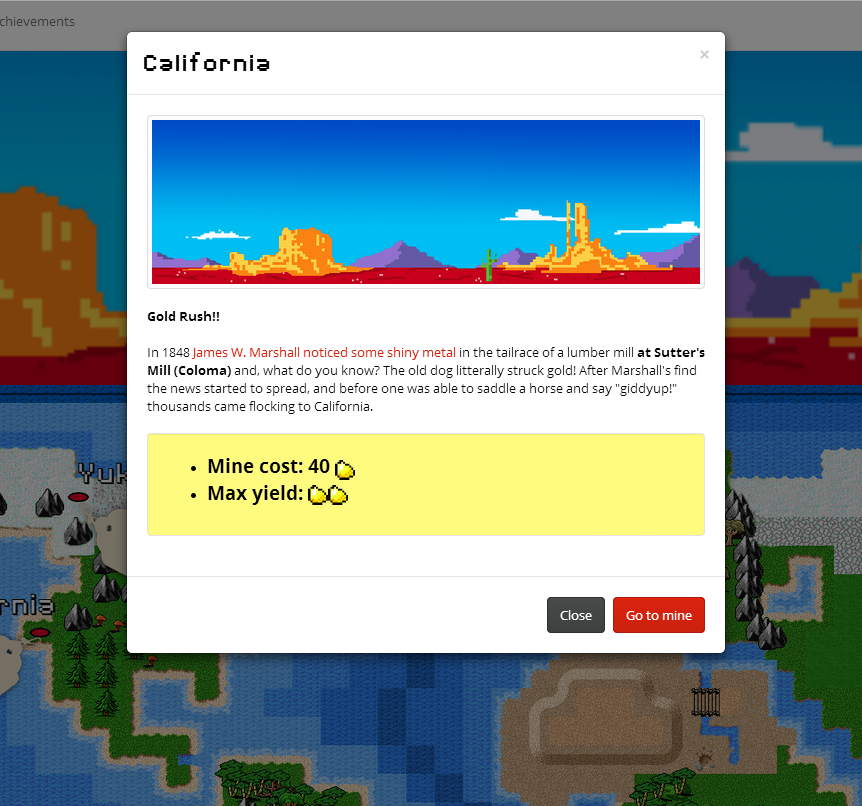
\includegraphics [width=1\textwidth] {cali.png}
        \end{subfigure}
\end{figure}

(1) Jill, the user, has just logged in (or registered) and has been redirected to the World Map. Her starting Equipment and Gold are as follows:
\begin{itemize}
	\item \textbf{Gold}: 100
  	\item \textbf{Scanning Tool}:  Oil Lamp (accuracy: 20\%, visibility: 2)
  	\item \textbf{Digging Tool}: Spoon (dig cost: 5, gold extracted 30\%)
	\item \textbf{Vehicle}: Boots (move cost: 10)
\end{itemize} 

On the map, Jill clicks on California and a modal appears, from which she can see see that, although the mine doesn't yield much gold, it is relatively cheap to access it (she only needs to pay 40 gold nuggets to enter it).

(2) After clicking on 'Go to Mine', 40 gold nuggets are removed from Jill's total amount of gold and she is presented with a mine where no layer has been dug. On the top left hand side Jill can see the name of the location she is in and the number of the mine (now 1) whereas on the right hand side she can check her total amount of gold (now 60) and the number of days she has been digging. Thanks to her Oil Lamp she can see specks of gold in the first two layers but, because the lamp only has a 20\% accuracy, it is possible that the amount of flecks that can be seen is deceiving. 
\begin{itemize}
	\item \textbf{Current gold}: 0
  	\item \textbf{Time remainingl}: 100
  	\item \textbf{Mine}: 1
	\item \textbf{Day}: 1
\end{itemize} 

(3) Jill decides to dig through the first couple of layers layer of the mine by clicking on the 'Move' button on the right hand side of the mine shaft. She gains 17 gold nuggets and consumes 10 units of time (since each digging operation costs 5 units of time)
\begin{itemize}
	\item \textbf{Current gold}: 17
  	\item \textbf{Time remainingl}: 90
  	\item \textbf{Mine}: 1
	\item \textbf{Day}: 1
\end{itemize} 

(4) At this point Jill is not sure she might get much more gold from this mine and she doesn't want to spend precious time digging through layers of the mine that she has no information about. For this reason she clicks on 'Move' to get to a new mine (in the same location). To do this she must spend 10 units of time
\begin{itemize}
	\item \textbf{Current gold}: 17
  	\item \textbf{Time remainingl}: 80
  	\item \textbf{Mine}: 2
	\item \textbf{Day}: 1
\end{itemize} 

\begin{figure}[!h]
        \centering
        \begin{subfigure} [h] {0.6\textwidth}
                \centering
                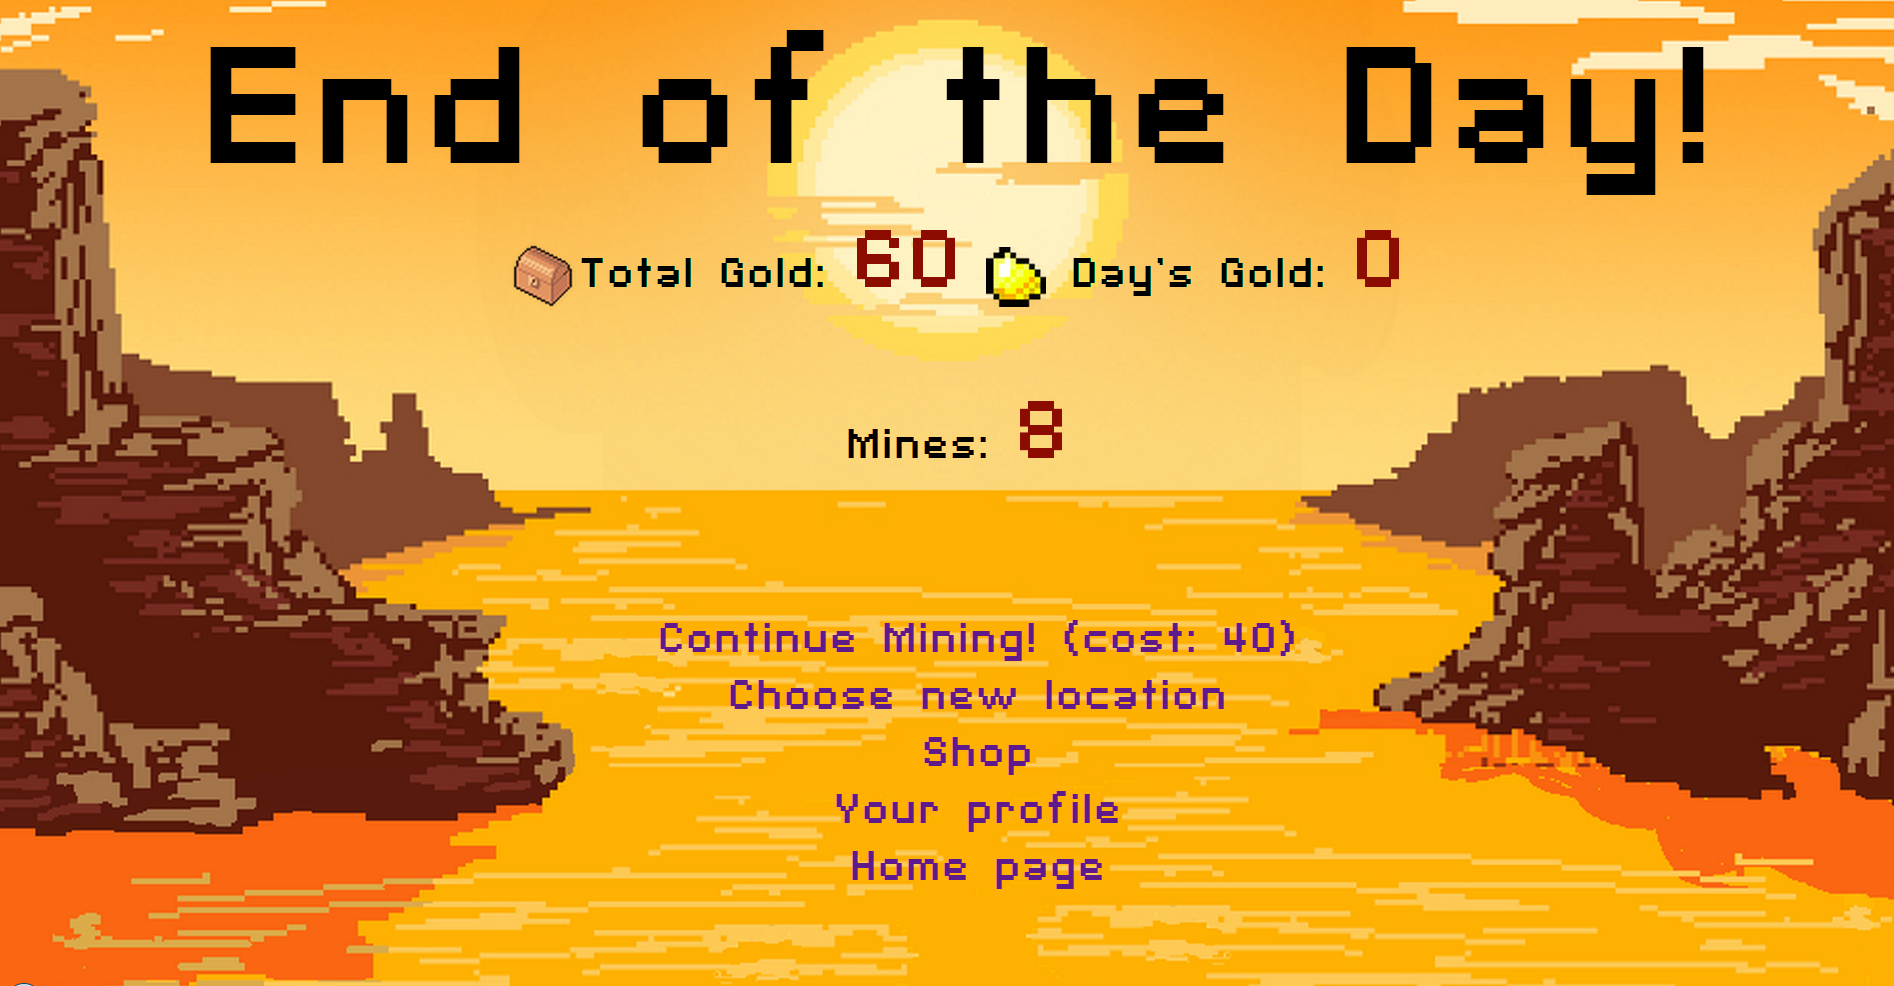
\includegraphics [width=1\textwidth] {endofday.png}
        \end{subfigure}
        \space
        \space
        \begin{subfigure} [h] {0.2\textwidth}
                \centering
                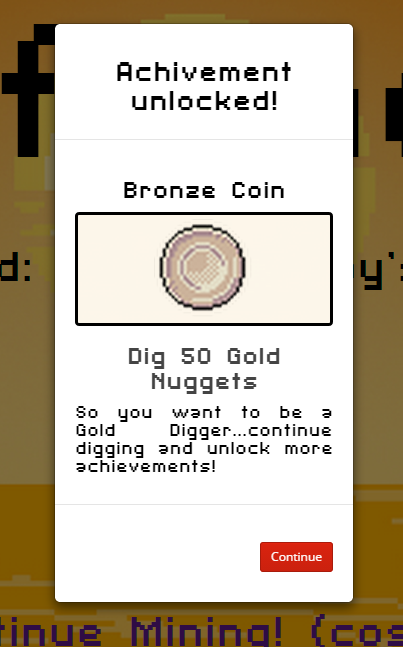
\includegraphics [width=1\textwidth] {bronze.png}
        \end{subfigure}
\end{figure}

(5) Jill continues to dig through some more mines and after a while she runs out of units of time. At this point, she is presented with the 'End of the Day' screen that sums up her progress during the day as follows:
\begin{itemize}
	\item \textbf{Today's gold}: 94 
  	\item \textbf{Total gold}: 94
  	\item \textbf{Mines dug}: 6 
\end{itemize} 
Jill also receives the 'Bronze Coin' achievement for having dug more than 50 gold nuggets. From here Jill decides to go to the shop and see if she can purchase some new items

\begin{figure}[!h]
        \centering
        \begin{subfigure} [h] {0.6\textwidth}
                \centering
                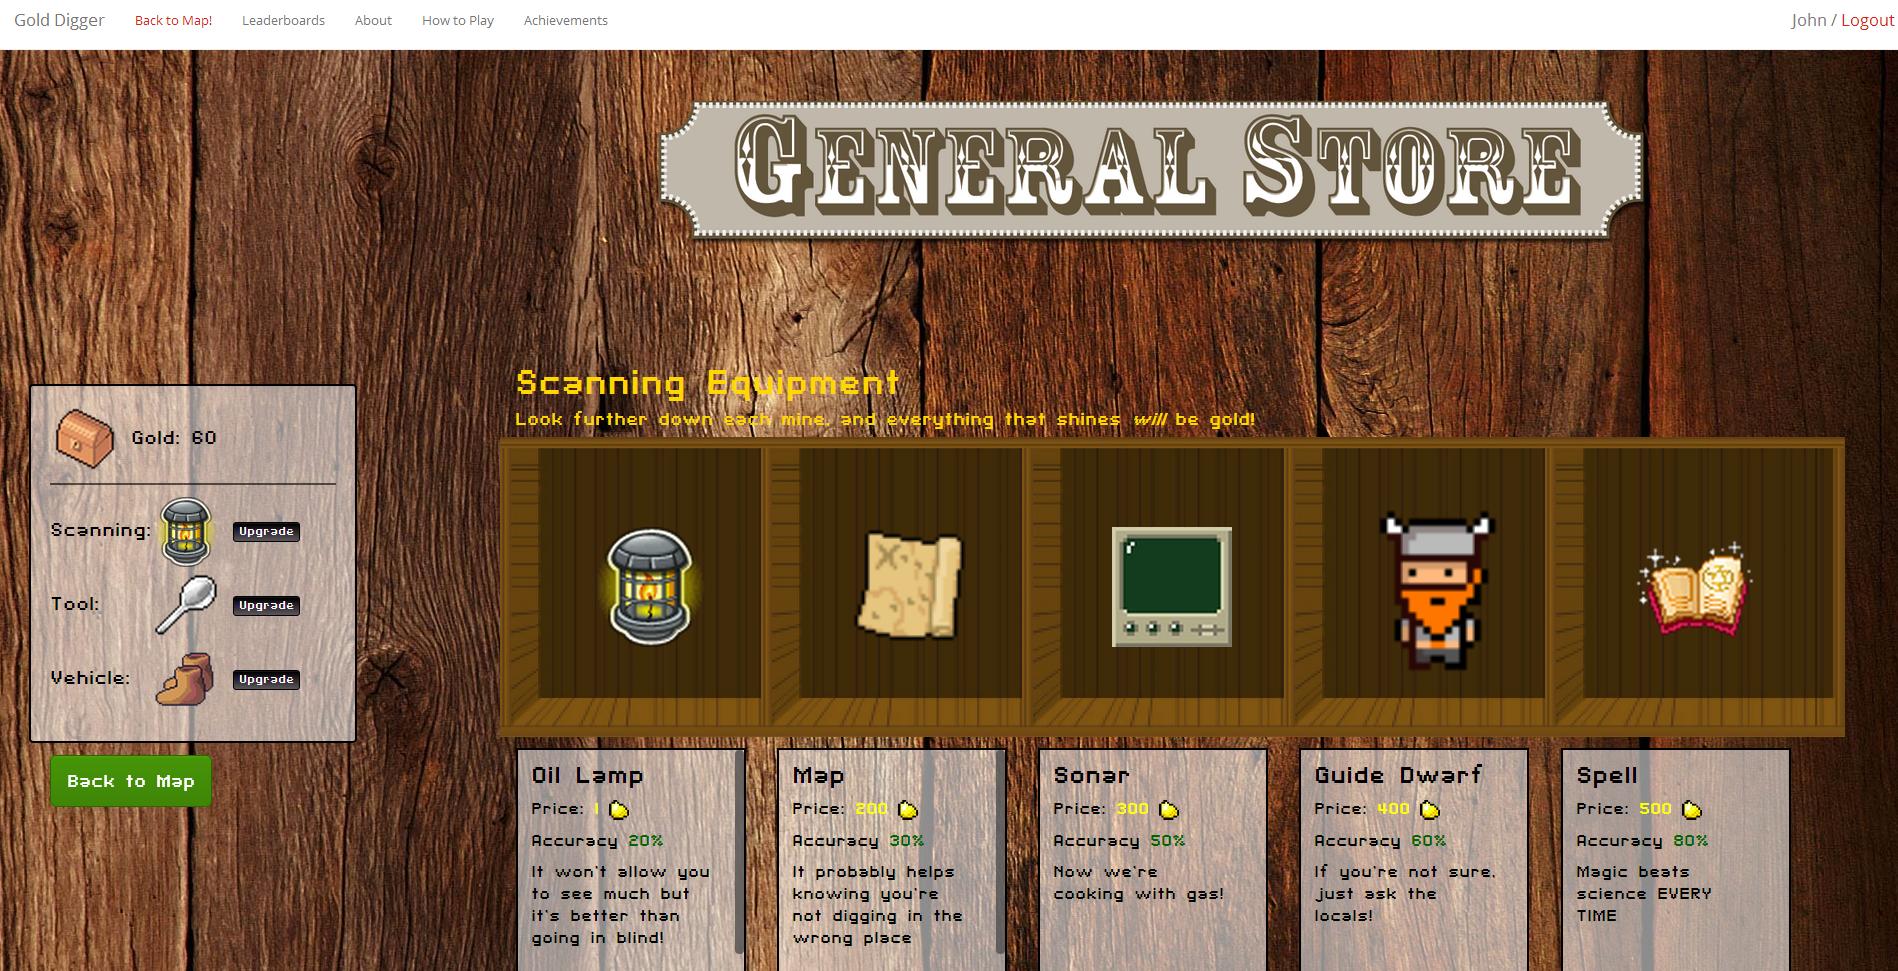
\includegraphics [width=1\textwidth] {generalstore.png}
        \end{subfigure}
        \space
        \space
        \begin{subfigure} [h] {0.3\textwidth}
                \centering
                
\includegraphics [width=1\textwidth] {nogold.png}
        \end{subfigure}
\end{figure}

(6) Once in the shop Jill tries to purchase better scanning equipment, so she clicks on the 'Upgrade' button next to the Oil Lamp. Unfortunately she doesn't have enough gold to make this purchase yet, so a message alerts her that she would need to do some more mining if she wants to be able to purchase the item.

\begin{figure}[!h]
        \centering
        \begin{subfigure} [h] {0.6\textwidth}
                \centering
                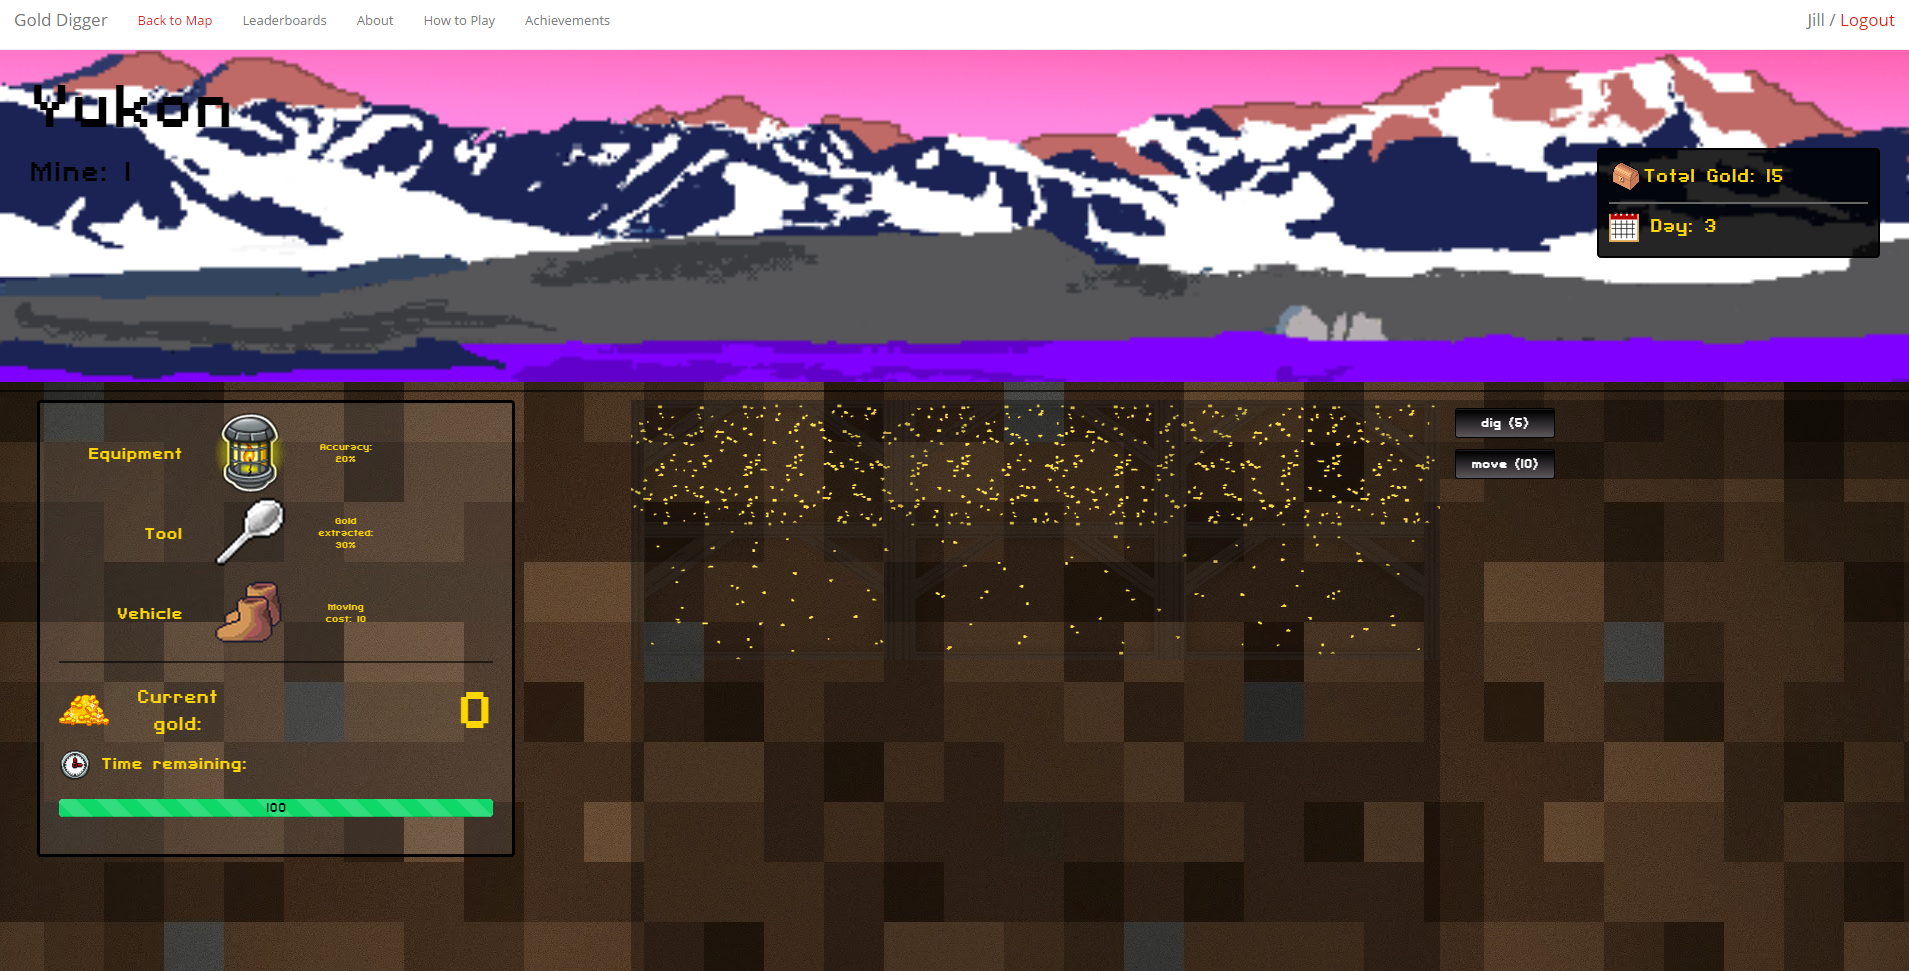
\includegraphics [width=1\textwidth] {yukon.png}
        \end{subfigure}
        \space
        \space
        \begin{subfigure} [h] {0.3\textwidth}
                \centering
                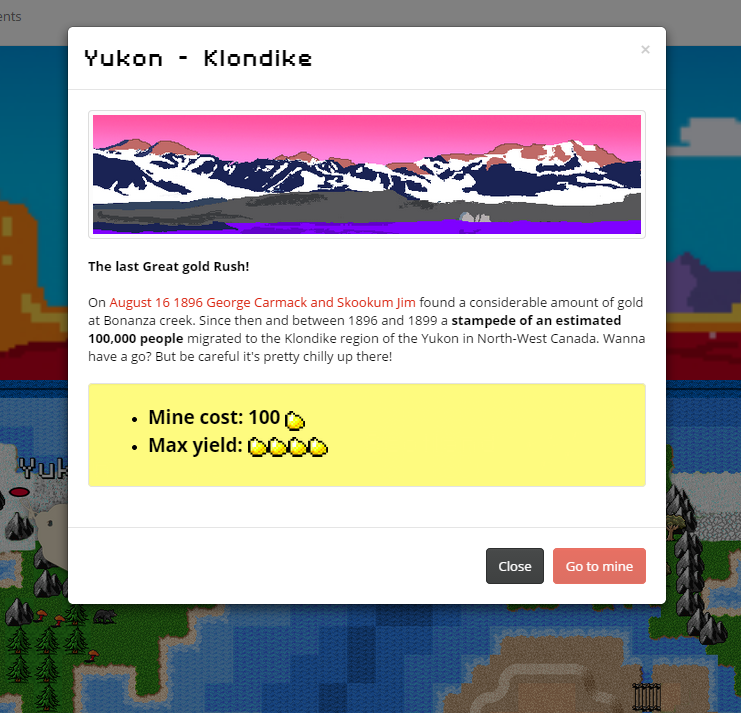
\includegraphics [width=1\textwidth] {yuki.png}
        \end{subfigure}
\end{figure}

(7) To gather more gold, Jill goes back to the California mines and, as soon as she has 100 gold nuggets, she takes a gamble and spends them on accessing the Yukon mine. However, she doesn't perform very well and, at the end of the day she owns less than 40 gold nuggets.
\begin{figure} [h] 
	\centering
           \makebox[\textwidth][c]{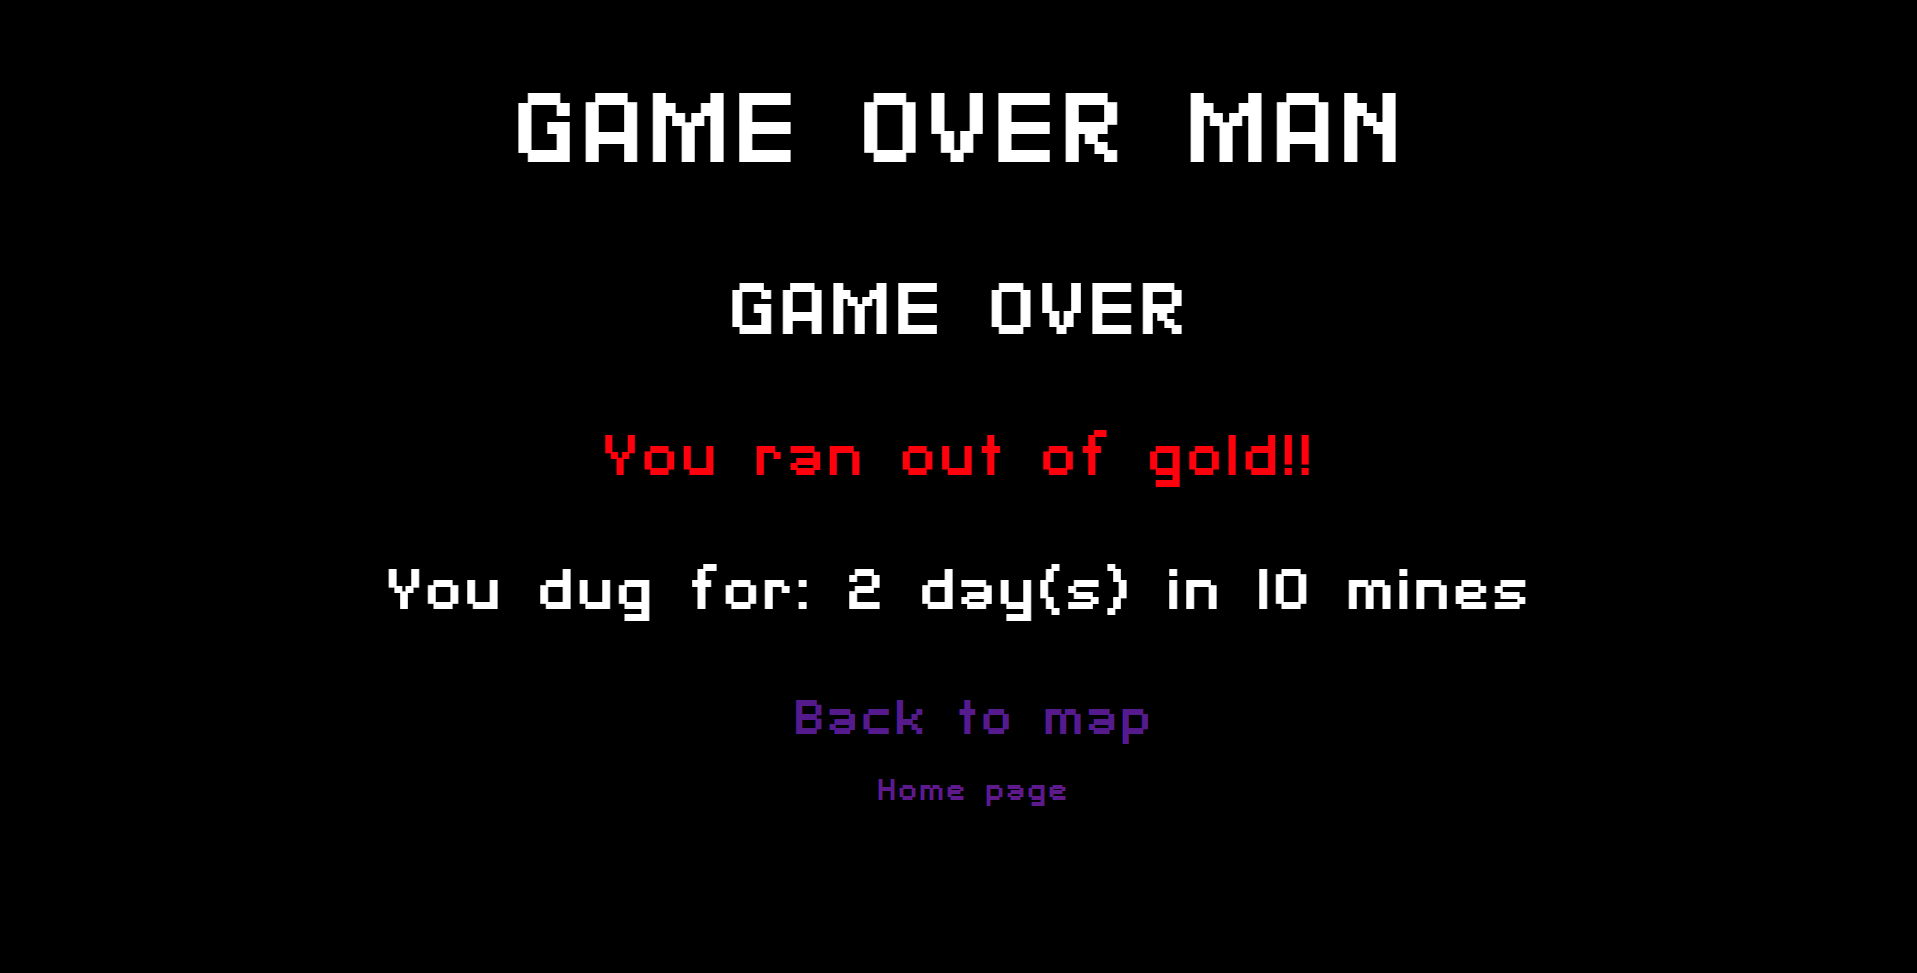
\includegraphics[width=1\textwidth]{gameover.png}}
\end{figure}
Because she doesn't have enough money to enter any of the mine, Jill loses her first game. However, clicking on 'Back to Map' will restore her to the initial conditions, if she bought any items they wold be lost.
\section{System Architechture}

\begin{figure} [h] 
	\centering
           \makebox[\textwidth][c]{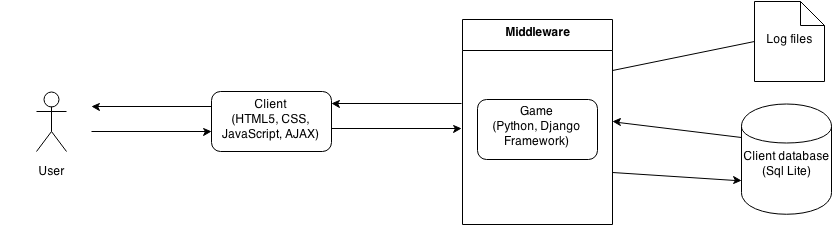
\includegraphics[width=1\textwidth]{architecture.png}}
\end{figure}

Gold Digger is based on a 3-tier architecture. Each user is able to create a player account (client) containing all of the details entered upon registration, together with a set of game variables, set to their starting values. The client side renders HTML5 and CSS3 elements and graphics while updates to the game states are done mostly through AJAX, in order to avoid reloading the page. The game logic is coded in the middleware using the python-based Django framework (see \ref {subsec:Django}). All of the user profiles as well as the other game objects and achievements are stored in the database while the corresponding graphics, as well as the rest of the game graphics are stored in the project's static and media folders. Finally, the middleware continuously updates a log file in order to monitor user behaviour and gather data to be parsed and analysed at a later stage.
\section{ER Model}

\begin{figure} [ht] 
	\centering
           \makebox[\textwidth][c]{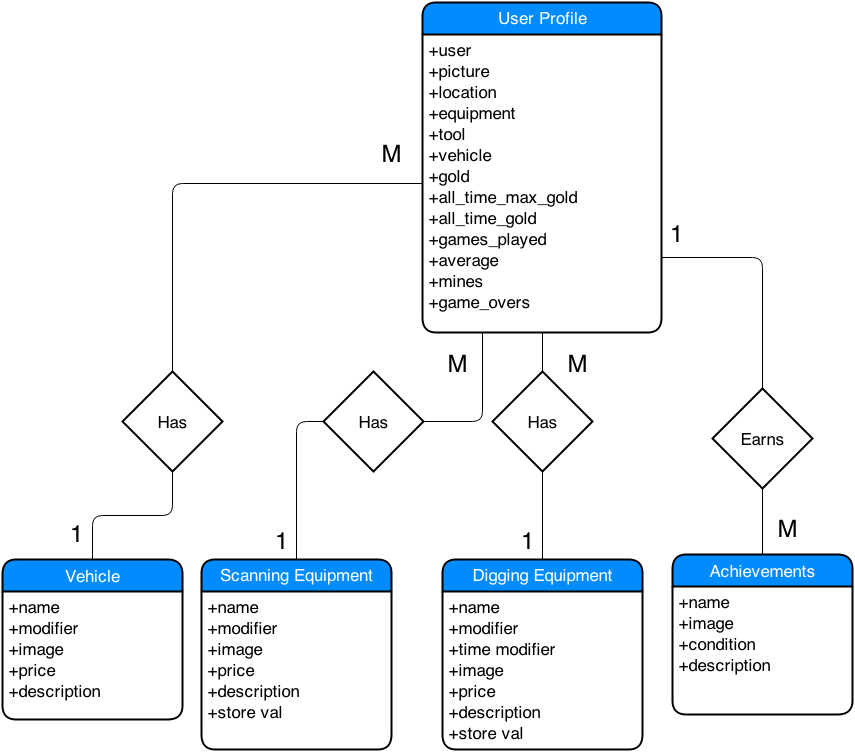
\includegraphics[width=0.7\textwidth]{er.png}}
	\caption{The Gold Digger ER diagram}
\end{figure}

The above diagram describes the entity-relationship model for Gold Digger. There are 5 entities in Gold Digger:
\begin{itemize}
	\item \textbf{User Profiles}: this entity contains several of the users' game stats, like the amount of gold at their disposal and the average amount of gold dug per mine as well as a reference to the Django object 'user' containing all the information regarding the user's password, username and email. This is necessary in order to take advantage of Django's very efficient user management system and keep the website as safe as possible 

  	\item \textbf{Digging Equipment}: this entity contains each of the tools' name, image, price and description. However, the most important attributes of this entity are the \textit{modifier} and the \textit{time modifier}. The\textit{modifier} attribute is used by the game mechanics to calculate how much gold a user is able to extract from a given layer of the mine. It is a \textit{float} number between 0.2 and 0.8  that will be multiplied by each of the amounts of gold in each layer. This way if the user is using, for instance, a shovel, she will be able to extract only 30\% of the gold that is actually present in that layer (see \ref{subsec:code}). The \textit{time modifier} attribute, on the other hand stores the digging cost per digging operation of each of the tools and it is an integer that goes from 5 to 1 in decreasing order from the worst tool to the best.

  	\item \textbf{Scanning Equipment}: this entity is quite similar to Digging Equipment but it does not include the \textit{time modifier} attribute. The \textit{modifier} attribute of this entity is responsible for calculating the cue array, that is in turn responsible for determining the amount of gold flecks that will be shown in each of the mine's layers (see \ref{subsec:code}). Furthermore, because this attribute holds only float values from 0.2 to 0.8, a simple multiplication by 10 is used  to determine the number of layers in which those specs are actually visible  .

	\item \textbf{Vehicles}: this entity, like Scanning Equipment, only posses the  \textit{modifier} attribute. This is an integer in range 10 to 6 and it holds the value of time units to be subtracted from the day's time, for each digging operation.  
	\item \textbf{Achievements}: the Achievement entity simply stores the name, image, condition and description of each of the achievements.
\end{itemize} 

\textbf{Relations}

There are \textbf{four relations} between the above entities. Each player can only store only one relation to a particular Scanning Equipment, Digging Equipment and Vehicle object thus, these are all one-to-one relationships. However, because each user can earn many achievements, the relationship between the User Profile and the Achievement entity needs a separate database table to keep track of the user-achievement value couples. In this table, \textbf{User Achievements}, each row comprises two columns, each of which is a foreign key. The first one is the relation to a User Profile Object, and the second one is the relation to an Achievement object.   

\section{Graphics}

One of the main elements of the design of Gold Digger was its graphic design. The general idea was to reproduce the look and feel of a retro 8-bit game as much as possible, without compromising the clarity and ease of use needed by a website. For this reason, 8-bit-style graphics were employed in most of the elements of the 'game pages' while Twitter Bootstrap was used in order to provide a simple minimalistic "framework" for the graphics to be displayed in. 

\textbf{Fonts}

There are two fonts that have been used throughout Gold Digger. The first one is \textbf{Open Sans} (see \ref{subsec: boot}). This font is part of the Twitter Bootstrap theme that provides the graphic framework for the site. It is used in areas with lots of text and in the navbar, where clarity the most important issue. However, throughout the site, most of the headings, scores, descriptions and game messages employ the font \textbf{SF Pixelate} (by ShyFonts) which has a pixelated look reminiscent of retro 8-bit games. All of the text in the 'game pages' is typed using this font. 

\textbf{Landscapes and World Map}

There are six different landscapes in Gold Digger, each one associated with one of the locations that the user can travel to and dig into. Three of them (California, Scotland and Yukon) were created with a pixel-art specific (Pixen) program using a number of pictures for inspiration, while the remaining three have been produced by applying filters, modifying and coloring similar pre-existing pictures in Photoshop CS, to achieve the 'pixelated look'. 

The World Map was created by importing a set of freeware game tiles into a freeware level design tool called 'Tiled' (see \ref{app: firstapp}). This tool allow users to load a particular set of tiles and arrange them on a grid of their choosing. The tileset used for the World Map was originally created for the expansion and creation of new maps for the game "Tales of Middle Earth" but it lent itself very well to the task of creating a word map. After the first version of the map was completed, the location names and price tags were added with Photoshop CS 6 where other minor adjustments were also made.

\textbf{Items and Achievements}

Most of the items and achievements icons were made by Alis, a pixel artist who made them available for public usage (see \ref{app: firstapp}). However a minor percentage of the items were created by modifying sprites of the popular game METAL SLUG  by SNK/Playmore. These sprites are all properties of their respective owners and no copyright is claimed upon them. 


%%%%%%%%%%%%%%%%%%%%%%%%%%%%%%%%%%%%%%%%%%%%%%%%%%%%%%%%%%%%%%%%%%%
\chapter{Impementation}
\label{implementation}
\section{Development Methods}
\section{Heuristic Evaluation}
\section{Testing}
\subsection{Unit Testing}
\subsection{Live Testing}
\section{Technologies}
\subsection{Django}
\label{subsec:Django}
\subsection{Python}
\subsection{HTML5}
\subsection{CSS3}
\paragraph{Animate.css}
\subsection{Twitter Bootstrap}
\label{subsec: boot}
\subsection{Javascript and JQuery}
\paragraph{Trip.js}
\paragraph{Animatenumbers.js}
\subsection{AJAX}
\subsection{Code}
\label{subsec:code}

%%%%%%%%%%%%%%%%%%%%%%%%%%%%%%%%%%%%%%%%%%%%%%%%%%%%%%%%%%%%%%%%%%%
\chapter{Results and Data}\label{results}
\section{Data Logged}
\section{Data Analysis}
\section{Results}
\section{Reflection}







%%%%%%%%%%%%%%%%%%%%%%%%%%%%%%%%%%%%%%%%%%%%%%%%%%%%%%%%%%%%%%%%%%%

\appendix % first appendix
%%%%%%%%%%%%%%%%%%%%%%%%%%%%%%%%%%%%%%%%%%%%%%%%%%%%%%%%%%%%%%%%%%%
\chapter{First appendix}
\label{app: firstapp}

\section{Section of first appendix}

%%%%%%%%%%%%%%%%%%%%%%%%%%%%%%%%%%%%%%%%%%%%%%%%%%%%%%%%%%%%%%%%%%%
\chapter{Second appendix}

%%%%%%%%%%%%%%%%%%%%%%%%%%%%%%%%%%%%%%%%%%%%%%%%%%%%%%%%%%%%%%%%%%%
% it is fine to change the bibliography style if you want

\bibliographystyle{plain}
\bibliography{mproj}
\nocite{*}
\end{document}
